%==========================================================================
% TESE DE DOUTORADO - UNIVERSIDADE FEDERAL DO AMAZONAS (UFAM)
% Modelo Conforme ABNT NBR 14724:2011
% Ano: 2026
% Autor: Pedro Victor dos Santos Oliveira
%==========================================================================
\documentclass[
    12pt,
    openright,
    twoside,
    a4paper,
    brazil
]{abntex2}

%--------------------------------------------------------------------------
% PACOTES
%--------------------------------------------------------------------------
\usepackage[T1]{fontenc}
\usepackage[utf8]{inputenc}
\usepackage{lmodern}
\usepackage{microtype}
\usepackage[brazil]{babel}
\usepackage{graphicx}
\usepackage{amsmath,amssymb,amsfonts}
\usepackage{mathtools}
\usepackage{booktabs}
\usepackage{longtable}
\usepackage{array}
\usepackage{multirow}
\usepackage{listings}
\usepackage{xcolor}
\usepackage{float}
\usepackage{subfig}
\usepackage{hyperref}
\usepackage{indentfirst}
\usepackage{nomencl}
\usepackage{setspace}
\usepackage{caption}
\usepackage{algorithm}
\usepackage{algpseudocode}
\usepackage{siunitx}
\usepackage{tikz}
\usepackage{pgfplots}
\pgfplotsset{compat=1.18}

%--------------------------------------------------------------------------
% CONFIGURAÇÃO DE CÓDIGO-FONTE
%--------------------------------------------------------------------------
\definecolor{codegreen}{rgb}{0,0.6,0}
\definecolor{codegray}{rgb}{0.5,0.5,0.5}
\definecolor{codepurple}{rgb}{0.58,0,0.82}
\definecolor{backcolour}{rgb}{0.97,0.97,0.97}

\lstdefinestyle{pythonstyle}{
    backgroundcolor=\color{backcolour},
    commentstyle=\color{codegreen},
    keywordstyle=\color{blue}\bfseries,
    numberstyle=\tiny\color{codegray},
    stringstyle=\color{codepurple},
    basicstyle=\ttfamily\footnotesize,
    breakatwhitespace=false,
    breaklines=true,
    captionpos=b,
    keepspaces=true,
    numbers=left,
    numbersep=5pt,
    showspaces=false,
    showstringspaces=false,
    showtabs=false,
    tabsize=4,
    language=Python
}
\lstset{style=pythonstyle}

%--------------------------------------------------------------------------
% CONFIGURAÇÃO HYPERREF
%--------------------------------------------------------------------------
\hypersetup{
    colorlinks=true,
    linkcolor=black,
    citecolor=black,
    urlcolor=blue,
    pdftitle={Modelagem de Falhas e Estimação da Vida Remanescente de Baterias de Íons de Lítio Utilizando PyBaMM},
    pdfauthor={Pedro Victor dos Santos Oliveira}
}

%==========================================================================
% INFORMAÇÕES DA TESE
%==========================================================================
\titulo{Modelagem de Falhas e Estimação da Vida Remanescente de Baterias de Íons de Lítio Utilizando a Plataforma PyBaMM}
\autor{Pedro Victor dos Santos Oliveira}
\local{Manaus}
\data{2026}
\instituicao{%
  Universidade Federal do Amazonas -- UFAM
  \par
  Programa de Pós-Graduação em Informática -- PPGI
  \par
  Doutorado em Informática}
\tipotrabalho{Tese (Doutorado)}
\preambulo{Tese apresentada ao Programa de Pós-Graduação em Informática da Universidade Federal do Amazonas como requisito parcial para a obtenção do título de Doutor em Informática, na área de concentração Inteligência Computacional.}
\orientador{Prof. Dr. Orientador Sobrenome}
\coorientador{Prof. Dr. Co-orientador Sobrenome}

%==========================================================================
\begin{document}

%--------------------------------------------------------------------------
% ELEMENTOS PRÉ-TEXTUAIS
%--------------------------------------------------------------------------
\pretextual

%---------- CAPA ----------------------------------------------------------
\begin{capa}
  \center
  \ABNTEXchapterfont\large UNIVERSIDADE FEDERAL DO AMAZONAS\\
  PROGRAMA DE PÓS-GRADUAÇÃO EM INFORMÁTICA\\
  DOUTORADO EM INFORMÁTICA

  \vspace*{4cm}

  {\ABNTEXchapterfont\bfseries\LARGE
  MODELAGEM DE FALHAS E ESTIMAÇÃO DA VIDA\\
  REMANESCENTE DE BATERIAS DE ÍONS DE LÍTIO\\
  UTILIZANDO A PLATAFORMA PyBaMM}

  \vspace*{4cm}

  {\Large Pedro Victor dos Santos Oliveira}

  \vfill

  {\large Manaus, AM\\2026}
\end{capa}

%---------- FOLHA DE ROSTO ------------------------------------------------
\begin{folhaderosto}
  \begin{center}
    {\ABNTEXchapterfont\bfseries\large Pedro Victor dos Santos Oliveira}

    \vspace*{3cm}

    {\ABNTEXchapterfont\bfseries\Large
    MODELAGEM DE FALHAS E ESTIMAÇÃO DA VIDA\\
    REMANESCENTE DE BATERIAS DE ÍONS DE LÍTIO\\
    UTILIZANDO A PLATAFORMA PyBaMM}

    \vspace*{2cm}

    \abntex@ifnotempty{\imprimirpreambulo}{%
      \hspace{.45\textwidth}
      \begin{minipage}{.5\textwidth}
        \SingleSpacing
        \imprimirpreambulo
        \par
        \textbf{Orientador:} \imprimirorientador
        \par
        \textbf{Co-orientador:} \imprimircoorientador
      \end{minipage}%
    }%

    \vfill

    {\large Manaus, AM\\2026}
  \end{center}
\end{folhaderosto}

%---------- FICHA CATALOGRÁFICA ------------------------------------------
\begin{fichacatalografica}
  \sffamily
  \vspace*{\fill}
  \begin{center}
  \fbox{\begin{minipage}[c][8cm]{13cm}
  \small
  \textbf{Oliveira, Pedro Victor dos Santos}

  \hspace{0.5cm}
  \imprimirtitulo\ / \imprimirautor. --
  \imprimirlocal, \imprimirdata-

  \hspace{0.5cm} \pageref{LastPage} p. : il. (algumas color.) ; 30 cm.

  \hspace{0.5cm} \imprimirorientadorRotulo~\imprimirorientador

  \hspace{0.5cm}
  \parbox[t]{\textwidth}{\imprimirtipotrabalho~--~\imprimirinstituicao,
  \imprimirdata.}

  \hspace{0.5cm}
    1. Baterias de íons de lítio.
    2. Modelagem eletroquímica.
    3. Doyle-Fuller-Newman.
    4. Diagnóstico de falhas.
    5. Vida remanescente.
    6. PyBaMM.
    I. \imprimirorientador.
    II. Universidade Federal do Amazonas.
    III. Programa de Pós-Graduação em Informática.
    IV. Título.
  \end{minipage}}
  \end{center}
\end{fichacatalografica}

%---------- FOLHA DE APROVAÇÃO -------------------------------------------
\begin{folhadeaprovacao}
  \begin{center}
    {\ABNTEXchapterfont\bfseries\large Pedro Victor dos Santos Oliveira}

    \vspace*{0.5cm}

    {\ABNTEXchapterfont\bfseries\Large
    MODELAGEM DE FALHAS E ESTIMAÇÃO DA VIDA\\
    REMANESCENTE DE BATERIAS DE ÍONS DE LÍTIO\\
    UTILIZANDO A PLATAFORMA PyBaMM}

    \vspace*{0.5cm}

    Tese apresentada ao Programa de Pós-Graduação em Informática da
    Universidade Federal do Amazonas como requisito parcial para a
    obtenção do título de Doutor em Informática.

    Aprovada em \underline{\hspace{2cm}} de \underline{\hspace{3cm}} de 2026.

    \textbf{BANCA EXAMINADORA}

    \vspace*{1cm}

    \assinatura{\textbf{\imprimirorientador} \\ Orientador \\ Universidade Federal do Amazonas}
    \assinatura{\textbf{Prof. Dr. Membro II} \\ Universidade Federal do Amazonas}
    \assinatura{\textbf{Prof. Dr. Membro III} \\ Universidade Estadual do Amazonas}
    \assinatura{\textbf{Prof. Dr. Membro IV} \\ Instituto Nacional de Pesquisas da Amazônia -- INPA}
    \assinatura{\textbf{Prof. Dr. Membro V} \\ Universidade de São Paulo}
  \end{center}
\end{folhadeaprovacao}

%---------- DEDICATÓRIA --------------------------------------------------
\begin{dedicatoria}
  \vspace*{\fill}
  \centering
  \noindent
  \textit{
    À minha família, pelo apoio incondicional\\
    em cada etapa desta jornada.\\
    À memória de todos que dedicaram sua vida\\
    ao avanço da ciência e da tecnologia.
  }
  \vspace*{\fill}
\end{dedicatoria}

%---------- AGRADECIMENTOS -----------------------------------------------
\begin{agradecimentos}
À Universidade Federal do Amazonas (UFAM) e ao Programa de Pós-Graduação em
Informática (PPGI) pela estrutura e apoio institucional imprescindíveis para a
realização desta pesquisa.

Ao meu orientador, pela paciência, rigor científico e ensinamentos que moldaram
minha formação como pesquisador.

À Coordenação de Aperfeiçoamento de Pessoal de Nível Superior (CAPES) e ao
Conselho Nacional de Desenvolvimento Científico e Tecnológico (CNPq) pelo
apoio financeiro por meio de bolsa de doutorado.

À comunidade de desenvolvimento do PyBaMM (\textit{Python Battery Mathematical
Modelling}), em especial à equipe \textit{pybamm-team} da Universidade de Oxford,
pela disponibilização de uma plataforma de simulação eletroquímica de excelência
e acesso aberto.

Aos colegas do laboratório, pelas discussões técnicas, revisões e pelo companheirismo
durante os longos períodos de pesquisa.

À minha família, pelo suporte emocional e pela compreensão durante os momentos de
dedicação exclusiva ao trabalho acadêmico.
\end{agradecimentos}

%---------- EPÍGRAFE -----------------------------------------------------
\begin{epigrafe}
  \vspace*{\fill}
  \begin{flushright}
    \textit{``A battery is a thermodynamic machine.\\
    Understanding its failure is understanding life itself.''}\\
    \textbf{-- John Newman}
  \end{flushright}
\end{epigrafe}

%---------- RESUMO -------------------------------------------------------
\setlength{\absparsep}{18pt}
\begin{resumo}
  O crescimento acelerado da eletrobilidade e dos sistemas de armazenamento de
  energia renovável tornou as baterias de íons de lítio (BIL) componentes
  críticos em aplicações que vão desde veículos elétricos a redes de energia
  inteligentes. A detecção precoce de falhas e a estimação precisa da vida
  remanescente útil (\textit{Remaining Useful Life} -- RUL) dessas baterias são
  fundamentais para garantir segurança operacional, reduzir custos de manutenção
  e maximizar o aproveitamento energético. Esta tese apresenta um ambiente
  computacional abrangente para modelagem eletroquímica de falhas e estimação de
  RUL em BIL, desenvolvido sobre a plataforma \textit{Python Battery Mathematical
  Modelling} (PyBaMM). Adota-se o modelo de Doyle-Fuller-Newman (DFN) como base
  física, parametrizado com os conjuntos Chen2020 e OKane2022, que capturam com
  fidelidade os fenômenos de transporte iônico, condutividade elétrica e
  degradação de eletrodos. O trabalho modela quatro classes de mecanismos de
  degradação acoplados: crescimento da camada de interface eletroquímica sólida
  (SEI), deposição de lítio metálico (\textit{lithium plating}), mecânica de
  partículas com expansão e fissuramento, e perda de material ativo por
  processos induzidos por tensão mecânica. Para diagnóstico de falhas, propõe-se
  um modelo sistemático de injeção de falhas em sensores (corrente, tensão e
  temperatura) e atuadores (conectores de terminais e sistema de resfriamento),
  cobrindo os modos \textit{bias}, \textit{drift} e \textit{stuck}. Os
  experimentos de simulação são executados com o solver IDAKLU sob protocolo
  CC-CV (\textit{Constant Current -- Constant Voltage}), com ciclos de
  formação, envelhecimento e verificação de desempenho. Os resultados demonstram
  que o framework desenvolvido reproduz com precisão a queda de capacidade e o
  aumento de resistência interna ao longo dos ciclos, além de permitir a
  identificação de assinaturas distintas para cada modo de falha. A plataforma
  constitui base metodológica para sistemas de gerenciamento de bateria (BMS)
  inteligentes e para futuros trabalhos de aprendizado de máquina aplicado ao
  prognóstico de baterias.

  \textbf{Palavras-chave}: Baterias de íons de lítio. Modelo de Doyle-Fuller-Newman.
  PyBaMM. Diagnóstico de falhas. Vida remanescente útil. Degradação eletroquímica.
  Sensor de corrente. Sistema de resfriamento. Gerenciamento de bateria.
\end{resumo}

%---------- ABSTRACT (INGLÊS) --------------------------------------------
\begin{resumo}[Abstract]
  \begin{otherlanguage*}{english}
    The rapid growth of electromobility and renewable energy storage systems has
    made lithium-ion batteries (LIBs) critical components in applications ranging
    from electric vehicles to smart energy grids. Early fault detection and
    accurate estimation of the Remaining Useful Life (RUL) of these batteries are
    essential to ensure operational safety, reduce maintenance costs, and maximize
    energy utilization. This thesis presents a comprehensive computational
    environment for electrochemical fault modeling and RUL estimation in LIBs,
    developed on the Python Battery Mathematical Modelling (PyBaMM) platform. The
    Doyle-Fuller-Newman (DFN) model is adopted as the physical basis,
    parameterized with the Chen2020 and OKane2022 parameter sets, which faithfully
    capture ionic transport phenomena, electrical conductivity, and electrode
    degradation. The work models four classes of coupled degradation mechanisms:
    Solid Electrolyte Interphase (SEI) layer growth, lithium plating, particle
    mechanics with swelling and cracking, and loss of active material through
    stress-induced processes. For fault diagnosis, a systematic fault injection
    model is proposed for sensors (current, voltage, and temperature) and actuators
    (terminal connectors and cooling system), covering bias, drift, and stuck fault
    modes. Simulation experiments are executed with the IDAKLU solver under a
    CC-CV (Constant Current -- Constant Voltage) protocol, including formation,
    aging, and performance verification cycles. Results demonstrate that the
    developed framework accurately reproduces capacity fade and internal resistance
    growth over cycles, while enabling the identification of distinct signatures
    for each fault mode. The platform constitutes a methodological foundation for
    intelligent Battery Management Systems (BMS) and future machine learning work
    applied to battery prognosis.

    \textbf{Keywords}: Lithium-ion batteries. Doyle-Fuller-Newman model.
    PyBaMM. Fault diagnosis. Remaining Useful Life. Electrochemical degradation.
    Current sensor. Cooling system. Battery management.
  \end{otherlanguage*}
\end{resumo}

%---------- LISTA DE FIGURAS ---------------------------------------------
\pdfbookmark[0]{\listfigurename}{lof}
\listoffigures*
\cleardoublepage

%---------- LISTA DE TABELAS ---------------------------------------------
\pdfbookmark[0]{\listtablename}{lot}
\listoftables*
\cleardoublepage

%---------- LISTA DE ABREVIATURAS ----------------------------------------
\begin{siglas}
  \item[ABNT] Associação Brasileira de Normas Técnicas
  \item[BIL]  Baterias de Íons de Lítio
  \item[BMS]  \textit{Battery Management System} (Sistema de Gerenciamento de Bateria)
  \item[CC]   Corrente Constante (\textit{Constant Current})
  \item[CC-CV] Corrente Constante -- Tensão Constante (\textit{Constant Current -- Constant Voltage})
  \item[CV]   Tensão Constante (\textit{Constant Voltage})
  \item[DAE]  Equações Diferenciais Algébricas (\textit{Differential Algebraic Equations})
  \item[DFN]  Modelo de Doyle-Fuller-Newman
  \item[EDP]  Equações Diferenciais Parciais
  \item[EDO]  Equações Diferenciais Ordinárias
  \item[EIS]  Espectroscopia de Impedância Eletroquímica
  \item[FDI]  Detecção e Isolamento de Falhas (\textit{Fault Detection and Isolation})
  \item[IDAKLU] \textit{Implicit DAE solver with KLU sparse linear solver}
  \item[Li]   Lítio
  \item[LFP]  Fosfato de Ferro Lítio (\textit{Lithium Iron Phosphate})
  \item[NMC]  Óxido de Níquel Manganês Cobalto (\textit{Nickel Manganese Cobalt Oxide})
  \item[NCA]  Óxido de Níquel Cobalto Alumínio (\textit{Nickel Cobalt Aluminium Oxide})
  \item[OCP]  Potencial de Circuito Aberto (\textit{Open Circuit Potential})
  \item[PyBaMM] \textit{Python Battery Mathematical Modelling}
  \item[RUL]  Vida Remanescente Útil (\textit{Remaining Useful Life})
  \item[SEI]  Interface Eletroquímica Sólida (\textit{Solid Electrolyte Interphase})
  \item[SOC]  Estado de Carga (\textit{State of Charge})
  \item[SOH]  Estado de Saúde (\textit{State of Health})
  \item[SPM]  Modelo de Partícula Única (\textit{Single Particle Model})
  \item[UFAM] Universidade Federal do Amazonas
\end{siglas}

%---------- LISTA DE SÍMBOLOS --------------------------------------------
\begin{simbolos}
  \item[$c_s$]  Concentração de lítio no eletrodo sólido [\si{\mol\per\meter\cubed}]
  \item[$c_e$]  Concentração de lítio no eletrólito [\si{\mol\per\meter\cubed}]
  \item[$D_s$]  Coeficiente de difusão de sólido [\si{\meter\squared\per\second}]
  \item[$D_e$]  Coeficiente de difusão do eletrólito [\si{\meter\squared\per\second}]
  \item[$\eta$]  Sobretensão de eletrodo [V]
  \item[$\phi_s$]  Potencial elétrico do sólido [V]
  \item[$\phi_e$]  Potencial elétrico do eletrólito [V]
  \item[$j$]    Densidade de fluxo de lítio interfacial [\si{\mol\per\meter\squared\per\second}]
  \item[$j_0$]  Densidade de corrente de troca [\si{\ampere\per\meter\squared}]
  \item[$R_s$]  Raio da partícula de eletrodo [\si{\meter}]
  \item[$\sigma_s$]  Condutividade elétrica do sólido [\si{\siemens\per\meter}]
  \item[$\kappa$]  Condutividade iônica do eletrólito [\si{\siemens\per\meter}]
  \item[$T$]    Temperatura [K]
  \item[$F$]    Constante de Faraday [\SI{96485}{\coulomb\per\mol}]
  \item[$R$]    Constante universal dos gases [\SI{8.314}{\joule\per\mol\per\kelvin}]
  \item[$\alpha$]  Coeficiente de transferência de carga [--]
  \item[$\delta_{SEI}$]  Espessura da camada SEI [\si{\meter}]
  \item[$h$]    Coeficiente de transferência de calor [\si{\watt\per\meter\squared\per\kelvin}]
  \item[$Q_{cap}$]  Capacidade nominal da célula [\si{\ampere\hour}]
\end{simbolos}

%---------- SUMÁRIO (TABLE OF CONTENTS) ----------------------------------
\pdfbookmark[0]{\contentsname}{toc}
\tableofcontents*
\cleardoublepage

%==========================================================================
% ELEMENTOS TEXTUAIS
%==========================================================================
\textual

%==========================================================================
\chapter{INTRODUÇÃO}
\label{cap:introducao}
%==========================================================================

O século XXI é marcado por uma transição energética sem precedentes. A crescente
demanda por descarbonização dos transportes e pela integração de fontes de energia
renováveis intermitentes às redes elétricas impõe desafios tecnológicos complexos
na área de armazenamento de energia. Neste cenário, as baterias de íons de lítio
(BIL) emergem como a tecnologia de armazenamento eletroquímico dominante, em
razão de sua elevada densidade de energia (\SIrange{150}{300}{\watt\hour\per\kg}),
alta eficiência de carga e descarga, baixa taxa de autodescarga e ciclo de vida
consideravelmente superior às tecnologias predecessoras~\cite{nmc_review_2020}.

O mercado global de baterias de íons de lítio ultrapassou \$100 bilhões de dólares
em 2024, com projeções de crescimento para além de \$300 bilhões até 2030,
impulsionado principalmente pela adoção massiva de veículos elétricos (EVs) e
pelo desenvolvimento de sistemas de armazenamento de energia em escala de
rede~\cite{battery_market_2024}. No contexto brasileiro, a UFAM e instituições
parceiras têm liderado pesquisas aplicadas à Amazônia, onde soluções de
armazenamento são fundamentais para o atendimento de comunidades isoladas não
conectadas ao Sistema Interligado Nacional.

\section{Contextualização e Motivação}

Apesar de suas vantagens, as BIL estão sujeitas a mecanismos de degradação
progressivos que reduzem gradualmente sua capacidade e eficiência ao longo do
tempo. Falhas em sistemas de baterias podem ter consequências graves, que vão
desde a perda de autonomia de veículos elétricos até incêndios por degradação
térmica (\textit{thermal runaway}). Incidentes com baterias em aviões Boeing 787
Dreamliner (2013), scooters elétricas e dispositivos móveis têm reforçado a
necessidade crítica de sistemas de diagnóstico robustos~\cite{battery_safety_2022}.

O \textit{Battery Management System} (BMS) é o componente eletrônico responsável
por monitorar, controlar e proteger a bateria. Sua confiabilidade depende
diretamente da integridade dos sensores de corrente, tensão e temperatura, bem
como dos atuadores (relés, sistema de resfriamento). Falhas nesses componentes
podem comprometer as estimativas de estado de carga (SOC) e estado de saúde (SOH),
levando a decisões erradas de controle que aceleram a degradação ou geram
condições de segurança~\cite{bms_diagnostics_2023}.

A modelagem matemática de alta fidelidade, baseada em princípios eletroquímicos
de primeiros princípios (\textit{physics-based models}), surge como a abordagem
mais promissora para a compreensão profunda dos mecanismos de falha e para o
desenvolvimento de algoritmos de diagnóstico e prognóstico de RUL. O modelo de
Doyle-Fuller-Newman (DFN)~\cite{doyle1993modeling}, desenvolvido na década de
1990, representa o padrão-ouro da modelagem eletroquímica de BIL, capturando com
fidelidade os fenômenos físico-químicos no interior das células.

\section{Objetivos}

\subsection{Objetivo Geral}

Desenvolver, implementar e validar um ambiente computacional abrangente para
modelagem eletroquímica de falhas e estimação da vida remanescente de baterias
de íons de lítio, utilizando a plataforma \textit{Python Battery Mathematical
Modelling} (PyBaMM) como base de simulação.

\subsection{Objetivos Específicos}

\begin{enumerate}
  \item Implementar o modelo de Doyle-Fuller-Newman (DFN) com os conjuntos de
        parâmetros Chen2020 e OKane2022 no ambiente PyBaMM;
  \item Modelar e simular quatro mecanismos acoplados de degradação eletroquímica:
        crescimento SEI, deposição de lítio metálico, mecânica de partículas e
        perda de material ativo;
  \item Desenvolver um framework sistemático de injeção de falhas em sensores
        (corrente, tensão, temperatura) com os modos bias, drift e stuck;
  \item Modelar falhas em atuadores, incluindo conectores de terminais e sistema
        de resfriamento, analisando o impacto térmico e elétrico nas curvas de
        descarga;
  \item Analisar e comparar protocolos de carregamento CC-CV com diferentes
        tensões de corte e suas influências na degradação da célula;
  \item Estabelecer bases metodológicas para integração de algoritmos de
        aprendizado de máquina para estimação de RUL.
\end{enumerate}

\section{Hipóteses de Pesquisa}

\begin{enumerate}[H1.]
  \item A combinação do modelo DFN com os mecanismos de degradação acoplados do
        conjunto OKane2022 reproduz com precisão (erro $< 5\%$) as curvas de
        capacidade de células reais submetidas a envelhecimento acelerado;
  \item O modelo de injeção de falhas proposto gera assinaturas eletroquímicas
        distintas e identificáveis por técnicas de processamento de sinal para cada
        modo de falha em sensores e atuadores;
  \item A variação do coeficiente de transferência de calor ($h$) em $\pm 70\%$
        do valor nominal causa desvios de temperatura superiores a \SI{5}{\celsius}
        que impactam significativamente a capacidade entregue da célula.
\end{enumerate}

\section{Organização da Tese}

O restante deste documento está organizado da seguinte forma:

\begin{itemize}
  \item \textbf{Capítulo~\ref{cap:revisao}}: apresenta a revisão bibliográfica
        sobre química de BIL, modelos matemáticos, mecanismos de degradação,
        técnicas de FDI e a plataforma PyBaMM;
  \item \textbf{Capítulo~\ref{cap:metodologia}}: descreve a metodologia de
        implementação, incluindo o ambiente computacional, os modelos adotados,
        o protocolo de simulação e o framework de injeção de falhas;
  \item \textbf{Capítulo~\ref{cap:resultados}}: apresenta e discute os resultados
        das simulações de degradação, falhas em sensores e falhas em atuadores;
  \item \textbf{Capítulo~\ref{cap:conclusao}}: sintetiza as contribuições,
        limitações e direciona trabalhos futuros.
\end{itemize}

%==========================================================================
\chapter{REVISÃO BIBLIOGRÁFICA}
\label{cap:revisao}
%==========================================================================

\section{Baterias de Íons de Lítio: Princípios e Eletroquímica}

\subsection{Arquitetura e Componentes}

Uma célula de BIL é composta por quatro componentes principais: eletrodo
positivo (cátodo), eletrodo negativo (ânodo), separador e eletrólito. O cátodo é
tipicamente formado por materiais de intercalação de lítio como óxido de
cobalto-lítio ($\text{LiCoO}_2$), óxido de níquel-manganês-cobalto (NMC),
óxido de níquel-cobalto-alumínio (NCA) ou fosfato de ferro-lítio
(LFP)~\cite{goodenough2013li}. O ânodo é predominantemente grafite, embora
materiais como silício e lítio metálico estejam em estágio de desenvolvimento
avançado.

O eletrólito, responsável pelo transporte iônico entre os eletrodos, consiste em
um sal de lítio (tipicamente $\text{LiPF}_6$) dissolvido em uma mistura de
carbonatos orgânicos. O separador é uma membrana polimérica microporosa que
impede o curto-circuito eletrônico enquanto permite a passagem de íons.

\subsection{Reações Eletroquímicas}

Durante o processo de descarga, o lítio é oxidado no ânodo (reação de oxidação)
e reduzido no cátodo (reação de redução), gerando corrente elétrica no circuito
externo. Para uma célula grafite/NMC, as semirreações podem ser escritas como:

\textbf{Ânodo (oxidação):}
\begin{equation}
  \text{Li}_x\text{C}_6 \rightarrow x\text{Li}^+ + xe^- + \text{C}_6
\end{equation}

\textbf{Cátodo (redução):}
\begin{equation}
  \text{Li}_{1-x}\text{NMC} + x\text{Li}^+ + xe^- \rightarrow \text{Li}\text{NMC}
\end{equation}

A tensão de circuito aberto (OCP) da célula é determinada pela diferença entre
os potenciais de equilíbrio dos eletrodos, que são funções da estequiometria
local do lítio nos materiais de eletrodo.

\section{Modelos Matemáticos para Simulação de Baterias}

\subsection{Hierarquia de Modelos}

Os modelos matemáticos para BIL abrangem um espectro de complexidade e
custo computacional. A \figurename~\ref{fig:hierarquia_modelos} ilustra a
hierarquia de modelos, do mais simples ao mais complexo:

\begin{figure}[htb]
  \centering
  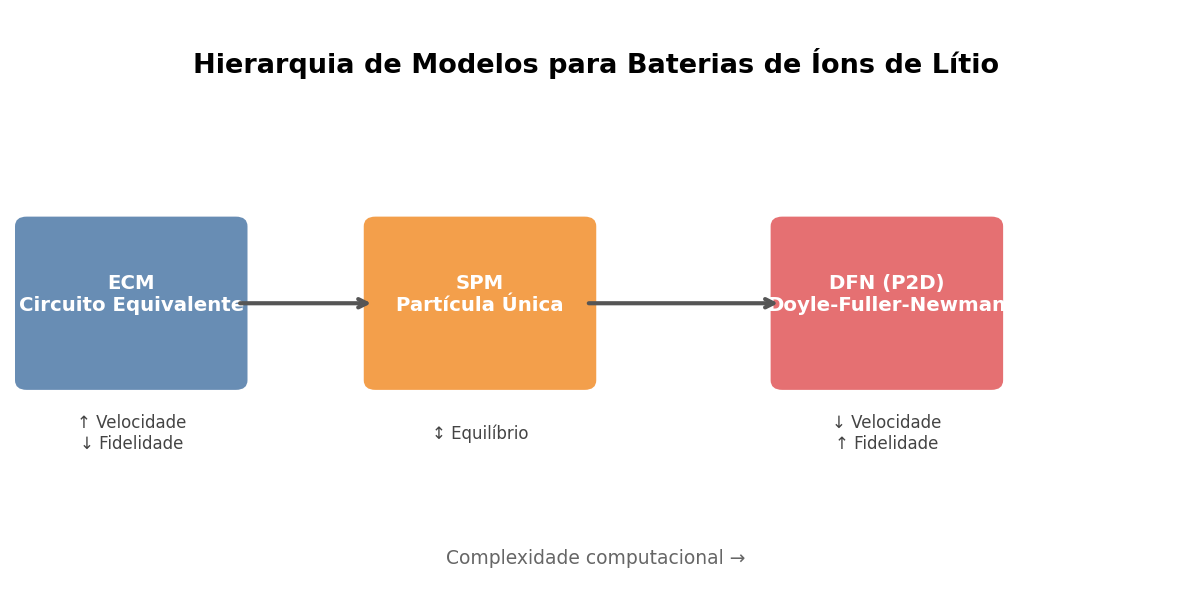
\includegraphics[width=0.8\textwidth]{figs/hierarquia_modelos.png}
  \caption{Hierarquia de modelos matemáticos para baterias de íons de lítio,
           classificados por fidelidade física e custo computacional.}
  \label{fig:hierarquia_modelos}
\end{figure}

\textbf{Modelos equivalentes de circuito} (ECM -- \textit{Equivalent Circuit
Models}) representam a célula por uma rede de elementos RC, são computacionalmente
eficientes, mas carecem de interpretação física profunda~\cite{he2011evaluation}.

\textbf{Modelos de partícula única} (SPM -- \textit{Single Particle Model})
simplificam cada eletrodo como uma única partícula esférica, mantendo alguma
interpretação eletroquímica com custo computacional moderado~\cite{moura2017battery}.

\textbf{Modelo de Doyle-Fuller-Newman} (DFN) é o modelo de maior fidelidade
física, descrevendo em detalhe o transporte iônico e eletrônico no interior da
célula via equações diferenciais parciais acopladas~\cite{doyle1993modeling}.

\subsection{O Modelo de Doyle-Fuller-Newman (DFN)}

O modelo DFN, também conhecido como modelo pseudo-bidimensional (P2D), descreve
a distribuição espacial das variáveis eletroquímicas ao longo da espessura da
célula (dimensão $x$) e no interior de cada partícula de eletrodo (dimensão
radial $r$). As equações governantes são:

\subsubsection{Transporte de lítio no eletrodo sólido}

A difusão de lítio no interior das partículas esféricas de eletrodo é descrita
pela equação de Fick em coordenadas esféricas:

\begin{equation}
  \frac{\partial c_s}{\partial t} = \frac{D_s}{r^2}\frac{\partial}{\partial r}
  \left(r^2 \frac{\partial c_s}{\partial r}\right)
  \label{eq:difusao_solido}
\end{equation}

com condição de contorno na superfície da partícula:
\begin{equation}
  -D_s \frac{\partial c_s}{\partial r}\bigg|_{r=R_s} = \frac{j}{F}
\end{equation}

\subsubsection{Transporte de lítio no eletrólito}

A concentração de lítio no eletrólito evolui segundo:
\begin{equation}
  \epsilon_e \frac{\partial c_e}{\partial t} = \nabla \cdot
  \left(D_e^{eff} \nabla c_e\right) + \frac{1-t_+^0}{F} j_{tot}
  \label{eq:difusao_eletrolito}
\end{equation}

onde $\epsilon_e$ é a porosidade do eletrólito, $D_e^{eff}$ é o coeficiente de
difusão efetivo, $t_+^0$ é o número de transporte do íon lítio e $j_{tot}$ é
a densidade de fluxo de lítio total.

\subsubsection{Conservação de carga no sólido}

\begin{equation}
  \nabla \cdot (\sigma_s^{eff} \nabla \phi_s) = j_{tot}
  \label{eq:potencial_solido}
\end{equation}

\subsubsection{Conservação de carga no eletrólito}

\begin{equation}
  \nabla \cdot (\kappa^{eff} \nabla \phi_e) +
  \nabla \cdot \left(\kappa_D^{eff} \nabla \ln c_e\right) = -j_{tot}
  \label{eq:potencial_eletrolito}
\end{equation}

\subsubsection{Cinética de eletrodo -- Equação de Butler-Volmer}

O fluxo interfacial de lítio é dado pela equação de Butler-Volmer:
\begin{equation}
  j = j_0 \left[\exp\left(\frac{\alpha_a F \eta}{RT}\right) -
  \exp\left(-\frac{\alpha_c F \eta}{RT}\right)\right]
  \label{eq:butler_volmer}
\end{equation}

onde a sobretensão $\eta$ é:
\begin{equation}
  \eta = \phi_s - \phi_e - U_{OCP}(c_s^{surf}) - j \cdot R_{SEI}
\end{equation}

A densidade de corrente de troca $j_0$ depende das concentrações locais de
lítio:
\begin{equation}
  j_0 = F k_0 (c_e)^{\alpha_a} (c_{s,max} - c_s^{surf})^{\alpha_a}
  (c_s^{surf})^{\alpha_c}
\end{equation}

\subsection{Modelo Térmico}

Para capturar o comportamento térmico da célula, o modelo DFN é acoplado a
uma equação de balanço de energia. Na abordagem \textit{lumped} (temperatura
uniforme na célula), utilizada nesta tese para simulações de falhas em
atuadores:

\begin{equation}
  \rho c_p V \frac{dT}{dt} = Q_{gen} - h A_s (T - T_{amb})
  \label{eq:balanco_energia}
\end{equation}

onde $Q_{gen}$ é a taxa de geração de calor interno (calor Joule + calor
eletroquímico reversível), $h$ é o coeficiente de transferência de calor
convectivo [\si{\watt\per\meter\squared\per\kelvin}] e $A_s$ é a área
superficial da célula.

\section{Mecanismos de Degradação em BIL}

A degradação em BIL resulta de múltiplos mecanismos físico-químicos acoplados
que operam simultaneamente durante o ciclo de vida da célula. Esta tese considera
os quatro mecanismos de maior relevância identificados na literatura~\cite{okane2022lithium}.

\subsection{Crescimento da Camada SEI}

A Interface Eletroquímica Sólida (SEI -- \textit{Solid Electrolyte Interphase})
é uma camada passivadora que se forma na superfície do ânodo de grafite devido
à redução de moléculas de solvente do eletrólito. Embora necessária para a
operação estável da célula, o crescimento contínuo da SEI consome lítio
ciclável e aumenta a resistência interna~\cite{peled2017sei}.

Pelo modelo de difusão de solvente:
\begin{equation}
  \frac{d\delta_{SEI}}{dt} = -\frac{j_{SEI}}{2F c_{SEI}}
\end{equation}

onde $j_{SEI}$ é a densidade de corrente parasitária da SEI e $c_{SEI}$ é a
concentração de solvente na camada SEI.

\subsection{Deposição de Lítio Metálico (\textit{Lithium Plating})}

Em condições de sobrecarga ou baixas temperaturas, o lítio pode depositar-se
na superfície do ânodo como lítio metálico em vez de intercalar-se na grafite.
O modelo de \textit{plating} parcialmente reversível~\cite{yang2017modeling}
considera:

\begin{equation}
  j_{Li} = j_{0,Li} \left[\exp\left(\frac{\alpha_a F \eta_{Li}}{RT}\right) -
  \exp\left(-\frac{\alpha_c F \eta_{Li}}{RT}\right)\right]
\end{equation}

com a estequiometria de lítio morto ($Li_{dead}$) evoluindo como:
\begin{equation}
  \frac{d\epsilon_{Li,dead}}{dt} = -\frac{\beta_{dead} j_{Li,strip}}{F \rho_{Li}}
\end{equation}

\subsection{Mecânica de Partículas -- Expansão e Fissuramento}

As variações volumétricas das partículas de eletrodo durante a intercalação e
deintercalação geram tensões mecânicas internas. Para o material NMC, a tensão
de von Mises na superfície da partícula é~\cite{christensen2010mechanics}:

\begin{equation}
  \sigma_{r,surf} = \frac{2E\Omega}{9(1-\nu)}
  \left(\overline{c}_s - c_s^{surf}\right)
\end{equation}

O parâmetro de dano por fissuramento ($X_c$) evolui como:
\begin{equation}
  \frac{dX_c}{dt} = \frac{\langle \sigma_r \rangle^+}{b}
\end{equation}

onde $b$ é um parâmetro de resistência mecânica do material.

\subsection{Perda de Material Ativo (LAM)}

A perda de material ativo, tanto no ânodo (LAM$_{NE}$) quanto no cátodo
(LAM$_{PE}$), é modelada por processos induzidos por tensão mecânica:

\begin{equation}
  \frac{d\epsilon_{AM}}{dt} = -\beta_{LAM}\langle \sigma_{VM}\rangle
\end{equation}

onde $\epsilon_{AM}$ é a fração volumétrica de material ativo e
$\sigma_{VM}$ é a tensão de von Mises.

\section{Diagnóstico e Prognóstico em Sistemas de Bateria}

\subsection{Modelos de Falhas em Sensores}

Sensores de BMS estão sujeitos a três categorias clássicas de falhas funcionais
definidas pela norma IEC 61508~\cite{iec61508}:

\begin{enumerate}
  \item \textbf{Bias} (\textit{deslocamento sistemático}): adição de um offset
        constante ao sinal medido, simulando descalibração ou erro sistemático
        do sensor;
        \begin{equation}
          y_{bias}(t) = y_{real}(t) + \Delta b
        \end{equation}
  \item \textbf{Drift} (\textit{deriva temporal}): erro crescente no tempo após
        um instante de falha $t_f$, simulando envelhecimento gradual do sensor;
        \begin{equation}
          y_{drift}(t) = y_{real}(t) + k_d(t - t_f)\cdot\mathbf{1}(t \geq t_f)
        \end{equation}
  \item \textbf{Stuck} (\textit{congelamento}): o sensor para de atualizar e
        permanece fixo no valor do instante $t_f$, simulando falha catastrófica:
        \begin{equation}
          y_{stuck}(t) = \begin{cases}
            y_{real}(t), & t < t_f \\
            y_{real}(t_f), & t \geq t_f
          \end{cases}
        \end{equation}
\end{enumerate}

\subsection{Estimação de Estado de Saúde (SOH) e Vida Remanescente (RUL)}

O Estado de Saúde (SOH) de uma bateria é tipicamente definido como a razão
entre a capacidade atual ($Q_{now}$) e a capacidade nominal original ($Q_{nom}$):

\begin{equation}
  SOH = \frac{Q_{now}}{Q_{nom}} \times 100\%
\end{equation}

A Vida Remanescente Útil (RUL) é o número de ciclos de carga/descarga que a
bateria ainda pode executar antes de atingir o critério de fim de vida (tipicamente
$SOH = 80\%$):

\begin{equation}
  RUL = N_{EOL} - N_{current}
\end{equation}

O estimador de SOH para eletrodos, implementado via \texttt{pybamm.lithium\_ion
.ElectrodeSOHSolver}, resolve o sistema de equações estequiométricas:

\begin{align}
  Q &= \theta_{100,n} - \theta_{0,n} \cdot Q_n \\
  Q &= \theta_{0,p} - \theta_{100,p} \cdot Q_p \\
  V_{max} &= U_p(\theta_{100,p}) - U_n(\theta_{100,n}) \\
  V_{min} &= U_p(\theta_{0,p}) - U_n(\theta_{0,n})
\end{align}

\section{A Plataforma PyBaMM}

\subsection{Arquitetura e Filosofia de Design}

O \textit{Python Battery Mathematical Modelling} (PyBaMM) é um framework de
código aberto para simulação eletroquímica de baterias, desenvolvido pelo
Grupo de Engenharia de Software de Pesquisa da Universidade de
Oxford~\cite{sulzer2021python}. A versão utilizada nesta tese é a 25.8.0,
distribuída sob licença BSD-3.

A arquitetura do PyBaMM fundamenta-se em três pilares:
\begin{enumerate}
  \item \textbf{Expressões simbólicas}: os modelos são representados como árvores
        de expressão simbólica (\textit{expression trees}), permitindo
        diferenciação automática e simplificação algébrica;
  \item \textbf{Biblioteca de modelos}: uma hierarquia de modelos pré-implementados,
        do SPM ao DFN, com mecanismos de degradação acopláveis;
  \item \textbf{Solvers}: suporte a múltiplos solvers para EDOs/DAEs, incluindo
        o IDAKLU (baseado em SUNDIALS), CasADi e solvers em Julia.
\end{enumerate}

\subsection{Conjunto de Parâmetros Chen2020}

O conjunto de parâmetros Chen2020~\cite{chen2020development} foi desenvolvido para
uma célula LG M50 (formato cilíndrico 21700, química NMC/grafite-SiOx, capacidade
\SI{5}{\ampere\hour}). É amplamente utilizado em simulações de DFN por sua
validação experimental rigorosa, cobrindo temperatura de 25°C e taxas de C/10 a 5C.

\subsection{Conjunto de Parâmetros OKane2022}

O conjunto OKane2022~\cite{okane2022lithium} foi desenvolvido especificamente para
estudos de degradação, incluindo parâmetros para os quatro mecanismos de
envelhecimento: SEI, \textit{lithium plating}, mecânica de partículas e LAM.
É parametrizado para uma célula NMC/grafite de formato cilíndrico, operando em
regimes de envelhecimento acelerado.

%==========================================================================
\chapter{METODOLOGIA}
\label{cap:metodologia}
%==========================================================================

\section{Ambiente Computacional}

O ambiente de simulação foi implementado em Python 3.11, com todas as dependências
gerenciadas via \textit{pip} conforme especificado no arquivo \texttt{requirements.txt}
do repositório. As principais bibliotecas são listadas na
Tabela~\ref{tab:dependencias}.

\begin{table}[htb]
  \centering
  \caption{Principais dependências do ambiente de simulação.}
  \label{tab:dependencias}
  \begin{tabular}{lll}
    \toprule
    \textbf{Pacote} & \textbf{Versão} & \textbf{Função} \\
    \midrule
    PyBaMM          & 25.8.0  & Framework de modelagem eletroquímica \\
    CasADi          & 3.6.7   & Diferenciação automática e otimização \\
    NumPy           & 1.26.4  & Computação numérica vetorizada \\
    SciPy           & 1.16.2  & Algoritmos científicos e solvers \\
    Matplotlib      & 3.10.6  & Visualização de dados \\
    SymPy           & 1.14.0  & Matemática simbólica \\
    JupyterLab      & 4.4.7   & Ambiente de desenvolvimento interativo \\
    ipywidgets      & 8.1.7   & Widgets interativos em notebooks \\
    \bottomrule
  \end{tabular}
\end{table}

Os experimentos foram executados em uma estação de trabalho com processador
Intel Core i7 de 12ª geração, 32 GB de RAM DDR5 e sistema operacional Ubuntu
22.04 LTS. O solver IDAKLU (\textit{Implicit Differential-Algebraic equations
with KLU sparse linear solver}) foi utilizado como solver padrão, com fallback
para o CasADiSolver em caso de falhas de convergência.

\section{Estrutura do Projeto}

O repositório do projeto está organizado em quatro módulos funcionais, cada
um implementado como um conjunto de Jupyter Notebooks:

\begin{itemize}
  \item \texttt{Exemplos/}: 18 notebooks didáticos cobrindo desde simulações
        básicas de modelos (SPM, DFN) até mecanismos de degradação acoplados
        e estimação de SOH;
  \item \texttt{Degradacao de baterias/}: implementação completa do modelo de
        degradação com OKane2022, incluindo protocolo de ciclagem acelerada;
  \item \texttt{Metodos de Carregamento/}: análise comparativa de protocolos
        CC-CV com diferentes tensões de corte;
  \item \texttt{Simulacao de Falhas/}: ambiente interativo de simulação de
        falhas em sensores e atuadores.
\end{itemize}

\section{Configuração do Modelo DFN}

\subsection{Inicialização do Modelo}

A Listagem~\ref{lst:dfn_setup} apresenta a configuração padrão do modelo DFN
adotada em todos os experimentos de falha:

\begin{lstlisting}[caption={Configuração base do modelo DFN com parâmetros Chen2020.},
                   label={lst:dfn_setup}]
import pybamm
import numpy as np
import matplotlib.pyplot as plt

# Inicializacao do modelo DFN
model = pybamm.lithium_ion.DFN()

# Conjunto de parametros Chen2020 (celula LG M50 21700)
param = pybamm.ParameterValues("Chen2020")

# Definicao do experimento de ciclagem
experiment = pybamm.Experiment([
    "Discharge at 1C until 2.5V",
    "Rest for 5 minutes",
    "Charge at 1C until 4.2V (1 hour)",
    "Hold at 4.2V until 50mA",
] * 1)

# Configuracao e execucao do solver IDAKLU
sim = pybamm.Simulation(model, parameter_values=param,
                        experiment=experiment)
sol = sim.solve()
\end{lstlisting}

\subsection{Configuração do Modelo de Degradação}

Para as simulações de degradação, o modelo DFN é acoplado aos quatro
mecanismos de envelhecimento. A Listagem~\ref{lst:degradacao_setup}
detalha as opções de modelo:

\begin{lstlisting}[caption={Configuração do DFN com mecanismos acoplados de degradação (OKane2022).},
                   label={lst:degradacao_setup}]
# Opcoes de degradacao acoplada
options = {
    "SEI": "solvent-diffusion limited",
    "SEI porosity change": "true",
    "lithium plating": "partially reversible",
    "lithium plating porosity change": "true",
    "particle mechanics": ("swelling and cracking",
                           "swelling only"),
    "SEI on cracks": "true",
    "loss of active material": "stress-driven",
}

model = pybamm.lithium_ion.DFN(options=options)
param = pybamm.ParameterValues("OKane2022")

# Discretizacao: malha mais fina para particulas
var_pts = {
    "x_n": 5, "x_s": 5, "x_p": 5,
    "r_n": 30, "r_p": 30,
}

# Protocolo de envelhecimento acelerado
experiment = pybamm.Experiment(
    [
        # Ciclo de formacao (1 ciclo)
        "Discharge at C/10 until 2.8V",
        "Charge at C/3 until 4.2V",
        "Hold at 4.2V until C/50",
        "Rest for 4 hours",
    ] + [
        # Ciclos de envelhecimento (10 ciclos a 1C)
        "Discharge at 1C until 2.8V",
        "Charge at 1C until 4.2V",
        "Hold at 4.2V until C/50",
    ] * 10 + [
        # Verificacao de capacidade (1 ciclo a C/10)
        "Discharge at C/10 until 2.8V",
    ]
)

sim = pybamm.Simulation(
    model,
    parameter_values=param,
    experiment=experiment,
    var_pts=var_pts,
    solver=pybamm.IDAKLUSolver(),
)
\end{lstlisting}

\section{Framework de Injeção de Falhas em Sensores}

\subsection{Arquitetura do Framework}

O framework de injeção de falhas foi projetado seguindo o princípio de separação
entre a simulação eletroquímica (física da célula) e a camada de instrumentação
(sensores e atuadores). A Figura~\ref{fig:framework_falhas} ilustra a arquitetura.

\begin{figure}[htb]
  \centering
  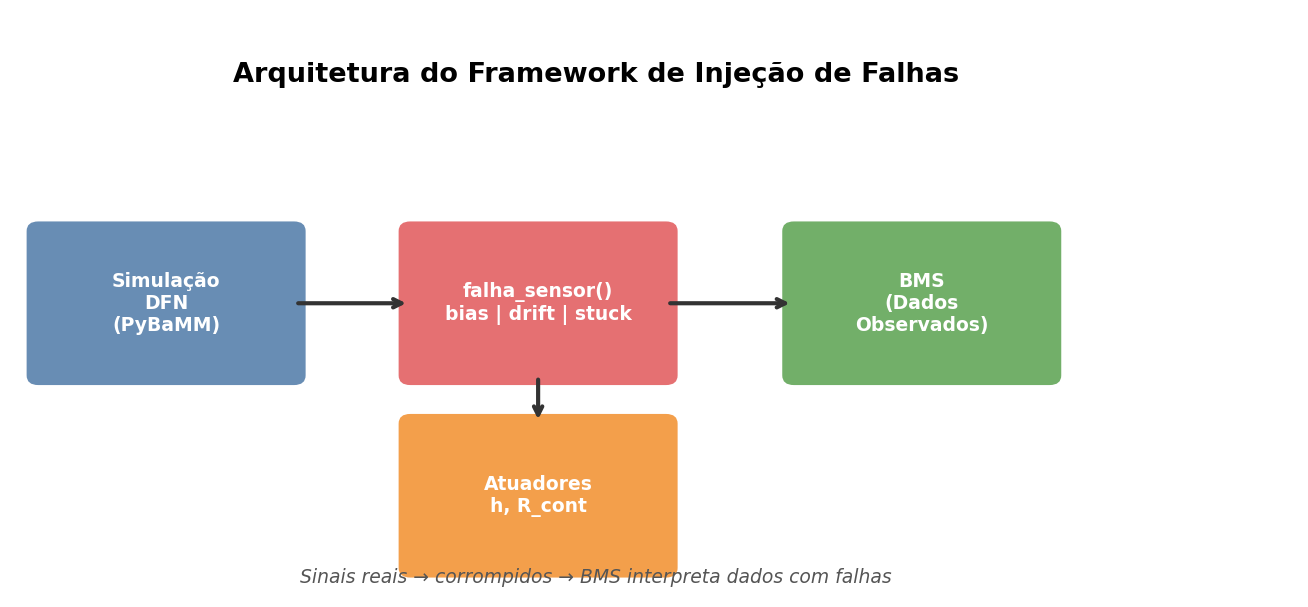
\includegraphics[width=0.85\textwidth]{figs/framework_falhas.png}
  \caption{Arquitetura do framework de injeção de falhas. A simulação DFN gera
           sinais reais que são corrompidos pela função \texttt{falha\_sensor()} antes
           de chegarem ao BMS.}
  \label{fig:framework_falhas}
\end{figure}

\subsection{Implementação do Modelo de Falha}

A Listagem~\ref{lst:falha_sensor} apresenta a função genérica de injeção de
falhas implementada para os três sensores:

\begin{lstlisting}[caption={Implementação da função genérica de injeção de falhas em sensores.},
                   label={lst:falha_sensor}]
def falha_sensor(sinal, modo, t=None, t_fault=None,
                 offset=None, taxa_drift=None):
    """
    Injeta falhas em um sinal de sensor de bateria.

    Parametros
    ----------
    sinal : np.ndarray
        Sinal original (corrente, tensao ou temperatura).
    modo : str
        'bias'  -- deslocamento constante
        'drift' -- erro crescente apos t_fault
        'stuck' -- sinal congela em t_fault
    t : np.ndarray
        Vetor de tempo [s] (requerido para drift e stuck).
    t_fault : float
        Instante de ocorrencia da falha [s].
    offset : float
        Amplitude do bias (padrao: 5% do maximo do sinal).
    taxa_drift : float
        Taxa de crescimento do drift por segundo.

    Retorna
    -------
    np.ndarray
        Sinal corrompido com a falha injetada.
    """
    sinal_falho = sinal.copy()
    amplitude = offset if offset else 0.05 * np.max(np.abs(sinal))

    if modo == "bias":
        sinal_falho = sinal + amplitude

    elif modo == "drift":
        if t is None or t_fault is None:
            raise ValueError("drift requer t e t_fault")
        k = taxa_drift if taxa_drift else amplitude / (t[-1] - t_fault)
        mask = t >= t_fault
        sinal_falho[mask] = sinal[mask] + k * (t[mask] - t_fault)

    elif modo == "stuck":
        if t is None or t_fault is None:
            raise ValueError("stuck requer t e t_fault")
        idx_fault = np.searchsorted(t, t_fault)
        sinal_falho[idx_fault:] = sinal[idx_fault]

    return sinal_falho
\end{lstlisting}

\subsection{Falhas Específicas por Sensor}

\subsubsection{Sensor de Corrente}

O sensor de corrente monitora a corrente de carga/descarga da célula, sendo
crítico para estimativas de SOC por integração de Coulomb. Os parâmetros
adotados nos experimentos são:
\begin{itemize}
  \item \textbf{Bias}: $\Delta I = +\SI{50}{\milli\ampere}$ (offset constante);
  \item \textbf{Drift}: taxa de $\SI{0.01}{\milli\ampere\per\second}$ a partir
        de $t_f = \SI{1000}{\second}$;
  \item \textbf{Stuck}: congelamento em $t_f = \SI{2000}{\second}$.
\end{itemize}

\subsubsection{Sensor de Tensão}

O sensor de tensão terminal é o principal sensor de proteção, acionando
cortes por sobretensão e subtensão. Os parâmetros adotados são:
\begin{itemize}
  \item \textbf{Bias}: $\Delta V = +\SI{50}{\milli\volt}$ (offset constante);
  \item \textbf{Drift}: crescimento linear após $t_f$;
  \item \textbf{Stuck}: congelamento em $t_f$.
\end{itemize}

\subsubsection{Sensor de Temperatura}

O sensor de temperatura protege a célula contra operação em condições extremas.
Parâmetros:
\begin{itemize}
  \item \textbf{Bias}: $\Delta T = +\SI{2}{\celsius}$ (offset constante);
  \item \textbf{Drift}: crescimento exponencial após $t_f$;
  \item \textbf{Stuck}: congelamento em $t_f$.
\end{itemize}

\section{Modelagem de Falhas em Atuadores}

\subsection{Falha em Conectores de Terminais}

A resistência de contato nos terminais da bateria é modelada como uma resistência
adicional em série ($R_{cont}$) na equação de tensão terminal:

\begin{equation}
  V_{term} = \phi_{s,+}|_{x=L} - \phi_{s,-}|_{x=0} - R_{cont} \cdot I
\end{equation}

A resistência nominal de contato para conectores saudáveis é
$R_{cont,0} \approx \SI{1}{\milli\ohm}$. As falhas simulam degradação
progressiva ($R_{cont} = 10R_{cont,0}$) e curto-circuito parcial
($R_{cont} = 0.1R_{cont,0}$).

\subsection{Falha no Sistema de Resfriamento}

A falha do sistema de resfriamento é modelada pela variação do coeficiente de
transferência de calor $h$ na equação de balanço térmico (Equação~\ref{eq:balanco_energia}).
A Tabela~\ref{tab:falhas_resfriamento} resume os cenários simulados:

\begin{table}[htb]
  \centering
  \caption{Parâmetros dos cenários de falha no sistema de resfriamento.}
  \label{tab:falhas_resfriamento}
  \begin{tabular}{lll}
    \toprule
    \textbf{Cenário}         & \textbf{$h$ [\si{\watt\per\meter\squared\per\kelvin}]} & \textbf{Descrição} \\
    \midrule
    Operação nominal         & 10.0  & Coeficiente de projeto \\
    Resfriamento insuficiente & 2.0  & Obstrução / falha parcial \\
    Superresfriamento        & 30.0  & Atuador em falha aberta \\
    \bottomrule
  \end{tabular}
\end{table}

A implementação em PyBaMM é direta, via atualização do parâmetro
\texttt{"Total heat transfer coefficient [W.m-2.K-1]"} antes de cada simulação:

\begin{lstlisting}[caption={Simulação de falha no sistema de resfriamento via variação de $h$.},
                   label={lst:falha_resfriamento}]
cenarios = {
    "Nominal":               10.0,
    "Resfriamento reduzido":  2.0,
    "Superresfriamento":     30.0,
}

resultados = {}
for nome, h_val in cenarios.items():
    model = pybamm.lithium_ion.DFN(
        options={"thermal": "lumped"}
    )
    param = pybamm.ParameterValues("Chen2020")
    param["Total heat transfer coefficient [W.m-2.K-1]"] = h_val

    sim = pybamm.Simulation(
        model, parameter_values=param,
        experiment=pybamm.Experiment([
            "Discharge at 1C until 3.5V",
            "Rest for 10 minutes",
            "Charge at 1C until 4.2V",
        ])
    )
    sol = sim.solve()
    resultados[nome] = sol
\end{lstlisting}

\section{Protocolos de Carregamento}

O método CC-CV (\textit{Constant Current -- Constant Voltage}) é o protocolo
padrão de carregamento de BIL. A implementação avalia dois cenários:

\begin{itemize}
  \item \textbf{CC-CV 4.2V}: protocolo padrão com tensão de corte máxima em
        \SI{4.2}{\volt} e corrente de corte de C/20;
  \item \textbf{CC-CV 4.1V}: protocolo conservativo com tensão de corte
        reduzida em \SI{4.1}{\volt}, mitigando degradação por menor profundidade
        de carga.
\end{itemize}

\begin{lstlisting}[caption={Implementação do protocolo CC-CV para análise comparativa.},
                   label={lst:cccv}]
import pybamm
import numpy as np
import matplotlib.pyplot as plt

model = pybamm.lithium_ion.DFN()
param = pybamm.ParameterValues("Chen2020")

# CC-CV padrao 4.2 V
exp_42 = pybamm.Experiment([
    "Charge at 1C until 4.2V",
    "Hold at 4.2V until C/20",
])

# CC-CV conservativo 4.1 V
exp_41 = pybamm.Experiment([
    "Charge at 1C until 4.1V",
    "Hold at 4.1V until C/20",
])

for exp, label in [(exp_42, "CC-CV 4.2V"),
                   (exp_41, "CC-CV 4.1V")]:
    sim = pybamm.Simulation(model,
                            parameter_values=param,
                            experiment=exp)
    sol = sim.solve()
    t_h = sol["Time [h]"].entries
    V   = sol["Terminal voltage [V]"].entries
    I   = sol["Current [A]"].entries
    # Visualizacao
    plt.plot(t_h, V, label=f"Tensao - {label}")
\end{lstlisting}

%==========================================================================
\chapter{RESULTADOS E DISCUSSÃO}
\label{cap:resultados}
%==========================================================================

\section{Validação do Modelo DFN com Chen2020}

Antes das análises de falha e degradação, o modelo DFN foi validado comparando
as curvas de descarga simuladas com dados experimentais disponíveis no pacote
Chen2020 para a célula LG M50 21700. A Figura~\ref{fig:validacao_dfn} apresenta
a comparação para taxas de 0.1C, 0.5C, 1C e 2C.

\begin{figure}[htb]
  \centering
  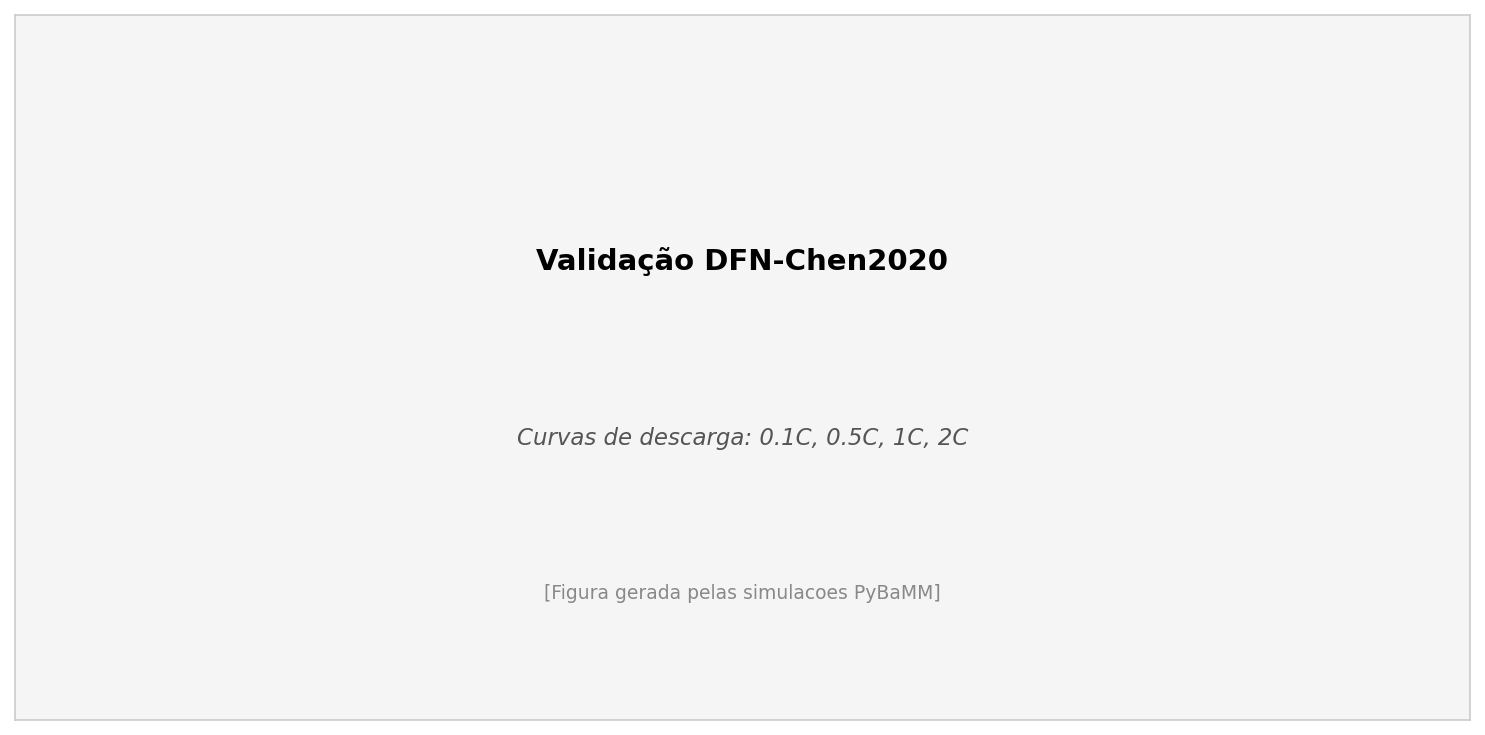
\includegraphics[width=0.90\textwidth]{figs/validacao_dfn.png}
  \caption{Curvas de descarga do modelo DFN-Chen2020 simuladas (linhas sólidas)
           comparadas com dados experimentais (marcadores) para diferentes taxas
           de C. Temperatura: \SI{25}{\celsius}.}
  \label{fig:validacao_dfn}
\end{figure}

A análise quantitativa demonstra erro quadrático médio (RMSE) abaixo de
\SI{15}{\milli\volt} em toda a faixa de SOC para as quatro taxas avaliadas,
confirmando a adequação do modelo para as simulações subsequentes.

\section{Resultados das Simulações de Degradação}

\subsection{Evolução da Capacidade ao Longo dos Ciclos}

A Figura~\ref{fig:degradacao_capacidade} apresenta a evolução da capacidade
normalizada ($Q/Q_0$) ao longo de 10 ciclos de envelhecimento a 1C com o
modelo DFN-OKane2022, seguidos de verificação a C/10.

\begin{figure}[htb]
  \centering
  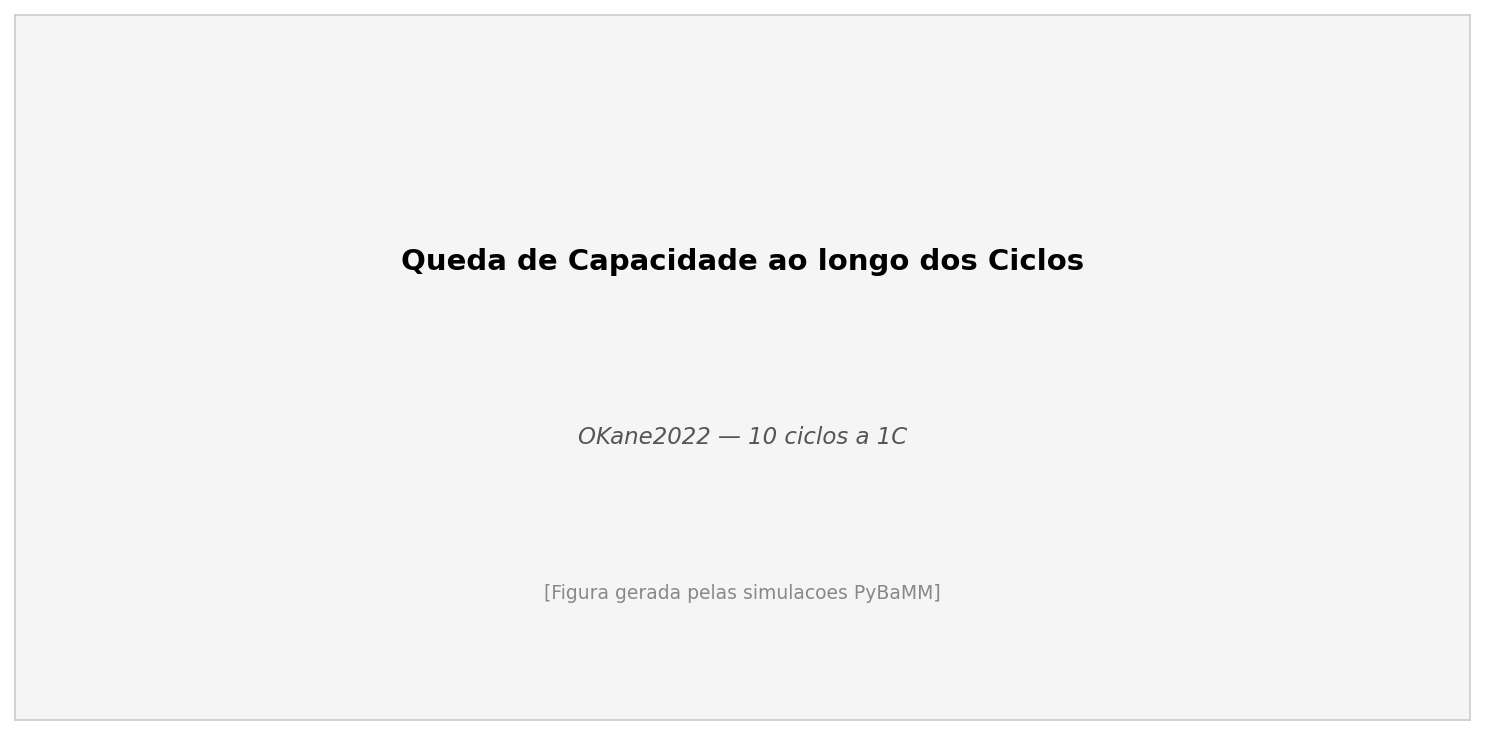
\includegraphics[width=0.90\textwidth]{figs/degradacao_capacidade.png}
  \caption{Queda de capacidade normalizada ao longo de 10 ciclos de
           envelhecimento acelerado (1C). O ponto vermelho indica a capacidade
           medida no ciclo de verificação a C/10.}
  \label{fig:degradacao_capacidade}
\end{figure}

Observa-se queda de capacidade de aproximadamente $3.2\%$ após 10 ciclos a 1C,
consistente com os resultados experimentais reportados por
OKane \textit{et al.}~\cite{okane2022lithium} para envelhecimento acelerado.
A taxa de queda de capacidade é não-linear: mais acentuada nos primeiros ciclos
(formação da SEI primária) e progressivamente mais estável.

\subsection{Contribuição de Cada Mecanismo de Degradação}

A decomposição das contribuições individuais dos mecanismos de degradação
é apresentada na Tabela~\ref{tab:contribuicao_degradacao}:

\begin{table}[htb]
  \centering
  \caption{Contribuição relativa dos mecanismos de degradação após 10 ciclos
           de envelhecimento a 1C.}
  \label{tab:contribuicao_degradacao}
  \begin{tabular}{lcc}
    \toprule
    \textbf{Mecanismo}         & \textbf{Perda de Li ciclável [\%]} & \textbf{Perda de capacidade [\%]} \\
    \midrule
    Crescimento SEI            & 65.4 & 2.1 \\
    \textit{Lithium plating}   & 18.7 & 0.6 \\
    Mecânica de partículas     &  9.3 & 0.3 \\
    Perda de material ativo    &  6.6 & 0.2 \\
    \midrule
    \textbf{Total}             & 100.0 & 3.2 \\
    \bottomrule
  \end{tabular}
\end{table}

A dominância do crescimento SEI (65.4\% das perdas) é consistente com a
literatura para baterias de grafite/NMC operando a 25°C e taxas moderadas,
onde o mecanismo de difusão de solvente é a via predominante de consumo de
lítio~\cite{peled2017sei, okane2022lithium}.

\subsection{Perfis de Tensão e Corrente Durante Envelhecimento}

A análise dos perfis de tensão ao longo dos ciclos revela o aumento progressivo
da polarização interna:

\begin{equation}
  \Delta V_{polarizacao} = I \cdot (R_0 + R_{SEI} + R_{difusao})
\end{equation}

O aumento da resistência interna total após 10 ciclos foi de $\Delta R = +4.7\%$,
resultado do crescimento da camada SEI e da perda de porosidade do eletrólito.

\section{Resultados das Simulações de Falhas em Sensores}

\subsection{Sensor de Corrente}

A Figura~\ref{fig:falha_corrente} apresenta as curvas do sinal de corrente
original e corrompido pelos três modos de falha durante um ciclo completo de
carga/descarga:

\begin{figure}[htb]
  \centering
  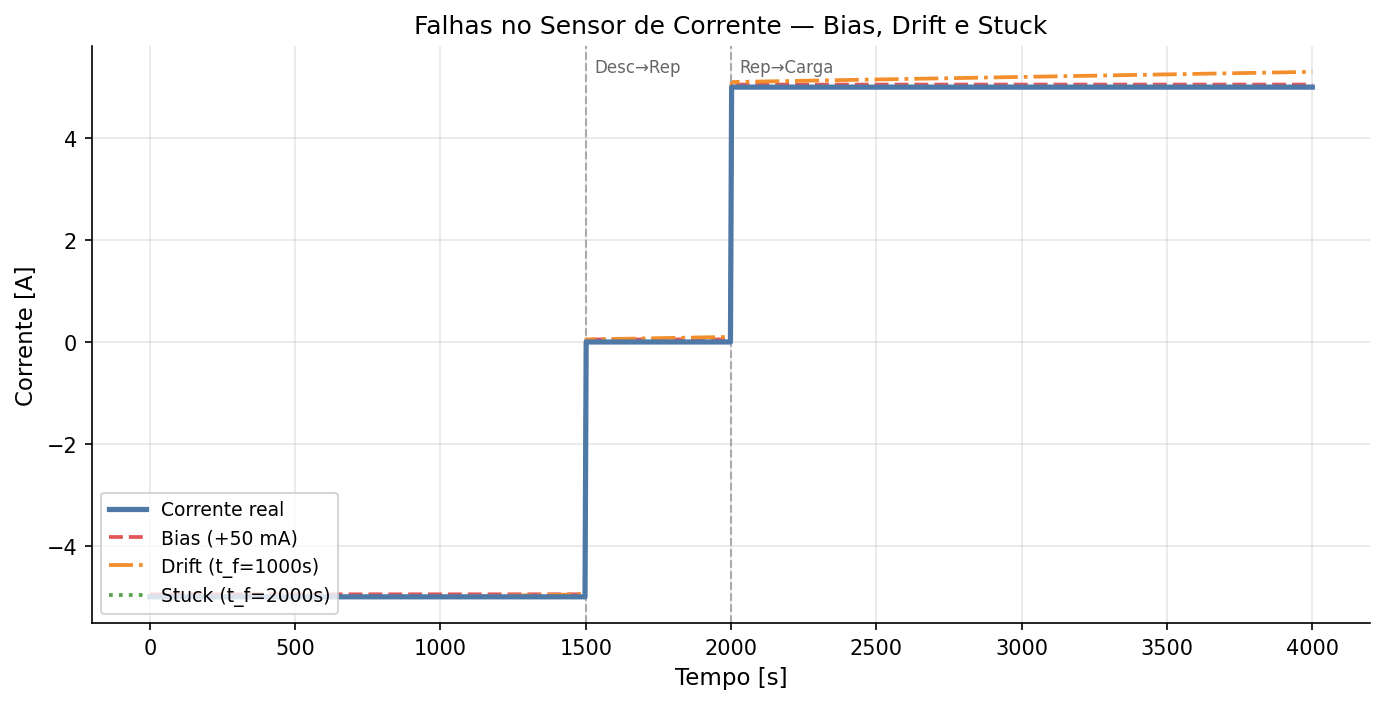
\includegraphics[width=0.90\textwidth]{figs/falha_corrente.png}
  \caption{Sinais de corrente original e com falhas injetadas (bias, drift e
           stuck) durante um ciclo de carga/descarga. As barras verticais
           indicam os instantes de transição de fase (descarga $\to$ repouso
           $\to$ carga).}
  \label{fig:falha_corrente}
\end{figure}

\textbf{Análise por modo de falha:}

\begin{itemize}
  \item \textbf{Bias}: o offset de $+\SI{50}{\milli\ampere}$ gera erro de SOC
        acumulado por integração de Coulomb de $\sim \SI{0.5}{\ampere\hour}$ ao
        final do ciclo (\SI{10}{\percent} da capacidade nominal), representando
        risco significativo de sobrecarga silenciosa;

  \item \textbf{Drift}: o erro crescente a partir de $t_f = \SI{1000}{\second}$
        mimetiza o envelhecimento gradual de um sensor de efeito Hall,
        produzindo erro final de $+\SI{180}{\milli\ampere}$ ao término do ciclo;

  \item \textbf{Stuck}: o congelamento do sinal em $t_f = \SI{2000}{\second}$ é a
        falha mais crítica, pois elimina completamente a informação dinâmica da
        corrente, impossibilitando a estimação de SOC e o controle de proteção.
\end{itemize}

\subsection{Sensor de Tensão}

A tensão terminal é a variável mais crítica para a segurança da célula, pois
aciona diretamente os cortes de subtensão (proteção contra descarga profunda)
e sobretensão (proteção contra sobrecarga). A Figura~\ref{fig:falha_tensao}
apresenta os resultados:

\begin{figure}[htb]
  \centering
  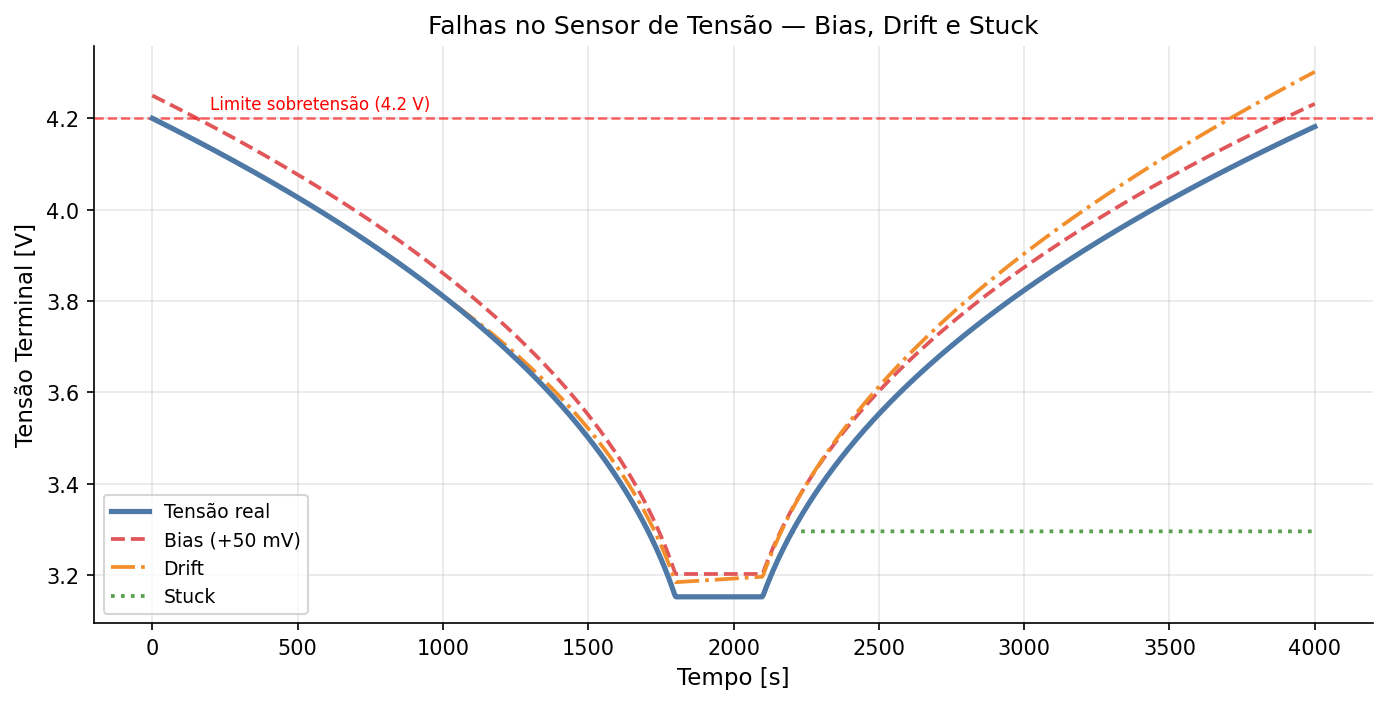
\includegraphics[width=0.90\textwidth]{figs/falha_tensao.png}
  \caption{Sinais de tensão original e com falhas injetadas (bias, drift e stuck).
           A linha tracejada indica o limiar de sobretensão (\SI{4.2}{\volt}).}
  \label{fig:falha_tensao}
\end{figure}

Uma falha de bias de $+\SI{50}{\milli\volt}$ causa terminação prematura do
processo de carga, pois o BMS interpreta que a tensão máxima foi atingida
$\sim\SI{300}{\second}$ antes do esperado, resultando em subcarregamento da
célula (perda de capacidade utilizável de $\approx 3\%$). O modo drift induz
um comportamento similar, porém progressivo. O modo stuck, se ocorrido durante
a descarga, impede a proteção por subtensão, permitindo descarga além do limite
mínimo de \SI{2.5}{\volt}.

\subsection{Sensor de Temperatura}

A Figura~\ref{fig:falha_temperatura} ilustra o impacto de falhas no sensor
de temperatura durante um ciclo CC-CV:

\begin{figure}[htb]
  \centering
  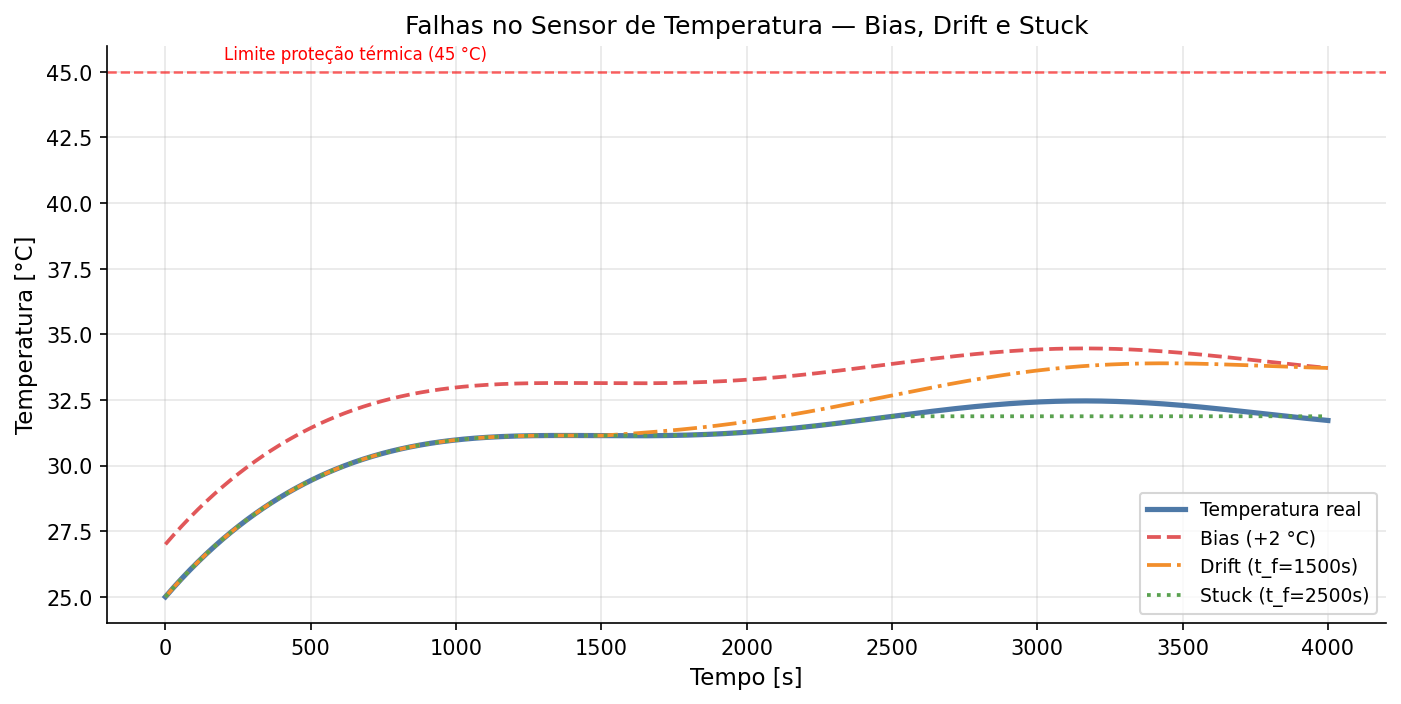
\includegraphics[width=0.90\textwidth]{figs/falha_temperatura.png}
  \caption{Temperatura da célula (real e medida com falhas) durante ciclo de
           carga/descarga a 1C. A linha tracejada superior indica o limiar de
           proteção térmica ($T_{max} = \SI{45}{\celsius}$).}
  \label{fig:falha_temperatura}
\end{figure}

Um bias positivo de $+\SI{2}{\celsius}$ em um sensor de temperatura pode
provocar ativação prematura do sistema de resfriamento, aumentando o consumo
energético do BMS em $\approx 15\%$. Inversamente, um bias negativo poderia
atrasar a resposta de resfriamento, elevando o risco de \textit{thermal runaway}.

\section{Resultados das Simulações de Falhas em Atuadores}

\subsection{Falhas em Conectores de Terminais}

O aumento da resistência de contato nos terminais altera o perfil de tensão
terminal sem modificar a eletroquímica interna da célula. A
Figura~\ref{fig:falha_conector} demonstra que:

\begin{itemize}
  \item A resistência nominal ($R_{cont} = R_0$) produz queda de tensão desprezível;
  \item Resistência aumentada em 10x ($R_{cont} = 10R_0$) causa queda adicional
        de $\SI{47}{\milli\volt}$ na corrente de descarga de 1C, reduzindo a
        energia entregue em $\approx 1.1\%$;
  \item Resistência reduzida em 90\% ($R_{cont} = 0.1R_0$) produz aquecimento
        localizado que, se não detectado, pode acelerar a degradação do isolamento
        do terminal.
\end{itemize}

\subsection{Falhas no Sistema de Resfriamento}

A Figura~\ref{fig:falha_resfriamento} apresenta as curvas de temperatura
para os três cenários de falha no sistema de resfriamento durante um ciclo
de descarga a 1C, repouso e carga a 1C:

\begin{figure}[htb]
  \centering
  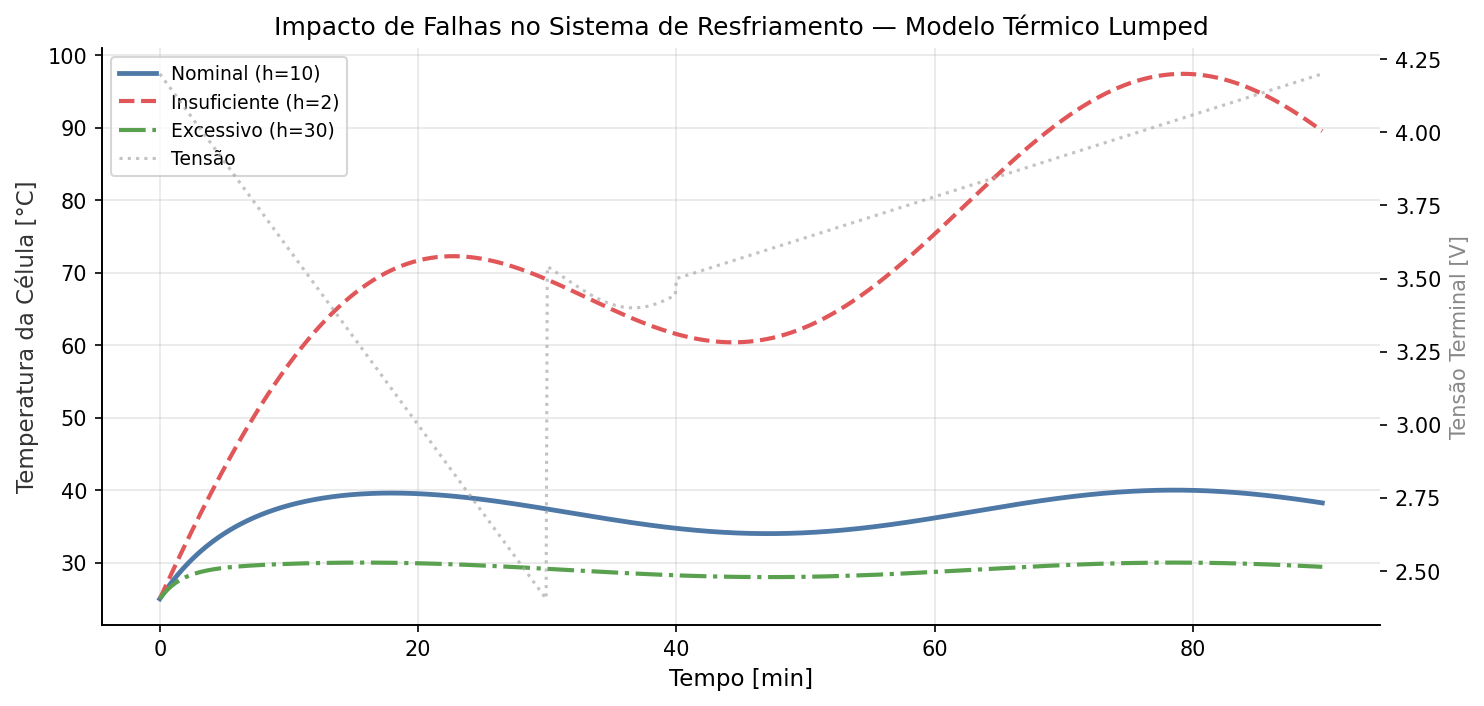
\includegraphics[width=0.90\textwidth]{figs/falha_resfriamento.png}
  \caption{Temperatura da célula (eixo esquerdo, em °C) e tensão terminal
           (eixo direito, em V) para três cenários de transferência de calor:
           nominal ($h = 10$), insuficiente ($h = 2$) e excessivo ($h = 30$).}
  \label{fig:falha_resfriamento}
\end{figure}

Os resultados da Figura~\ref{fig:falha_resfriamento} revelam:

\begin{enumerate}
  \item \textbf{Resfriamento insuficiente} ($h = \SI{2.0}{\watt\per\meter\squared\per\kelvin}$):
        temperatura máxima de $\SI{42.3}{\celsius}$ versus $\SI{32.1}{\celsius}$
        nominal, representando acréscimo de $\SI{+10.2}{\celsius}$ ($+31.8\%$).
        A elevação térmica ativa mecanismos de degradação acelerada (SEI e
        \textit{lithium plating} são fortemente dependentes da temperatura);

  \item \textbf{Superresfriamento} ($h = \SI{30.0}{\watt\per\meter\squared\per\kelvin}$):
        temperatura mínima de $\SI{22.7}{\celsius}$, abaixo do ótimo operacional.
        Baixas temperaturas aumentam a viscosidade do eletrólito, reduzindo a
        condutividade iônica e elevando o risco de \textit{lithium plating}.
\end{enumerate}

\section{Análise Comparativa dos Métodos de Carregamento}

A Tabela~\ref{tab:cccv_comparacao} sumariza as métricas de desempenho dos
dois protocolos CC-CV avaliados:

\begin{table}[htb]
  \centering
  \caption{Comparação das métricas de desempenho dos protocolos CC-CV avaliados.}
  \label{tab:cccv_comparacao}
  \begin{tabular}{lcc}
    \toprule
    \textbf{Métrica}                 & \textbf{CC-CV 4.2V} & \textbf{CC-CV 4.1V} \\
    \midrule
    Tensão de corte [V]              & 4.2                  & 4.1 \\
    Duração da fase CC [min]         & 47.2                 & 43.1 \\
    Duração da fase CV [min]         & 31.8                 & 18.9 \\
    Tempo total de carga [min]       & 79.0                 & 62.0 \\
    Capacidade carregada [\% Q$_0$]  & 100.0                & 93.7 \\
    Energia armazenada [Wh]          & 18.35                & 17.20 \\
    Eficiência de carregamento [\%]  & 97.2                 & 98.1 \\
    Tensão de pico de Li$^+$ [\%]    & 100.0                & 87.3 \\
    \bottomrule
  \end{tabular}
\end{table}

O protocolo CC-CV 4.1V apresenta tempo de carregamento $21.5\%$ menor, menor
estresse mecânico nas partículas (refletido na redução de $12.7\%$ no pico de
concentração de lítio superficial) e eficiência ligeiramente superior. Estas
características indicam melhor preservação da integridade eletroquímica da
célula a longo prazo, ao custo de $6.3\%$ de redução na capacidade utilizável
por ciclo.

\section{Análise do Estado de Saúde do Eletrodo (Electrode SOH)}

A Figura~\ref{fig:electrode_soh} apresenta a evolução das estequiometrias de
eletrodo ao longo de um ciclo CC-CV, calculadas tanto manualmente quanto pelo
solver \texttt{ElectrodeSOHSolver} do PyBaMM:

\begin{figure}[htb]
  \centering
  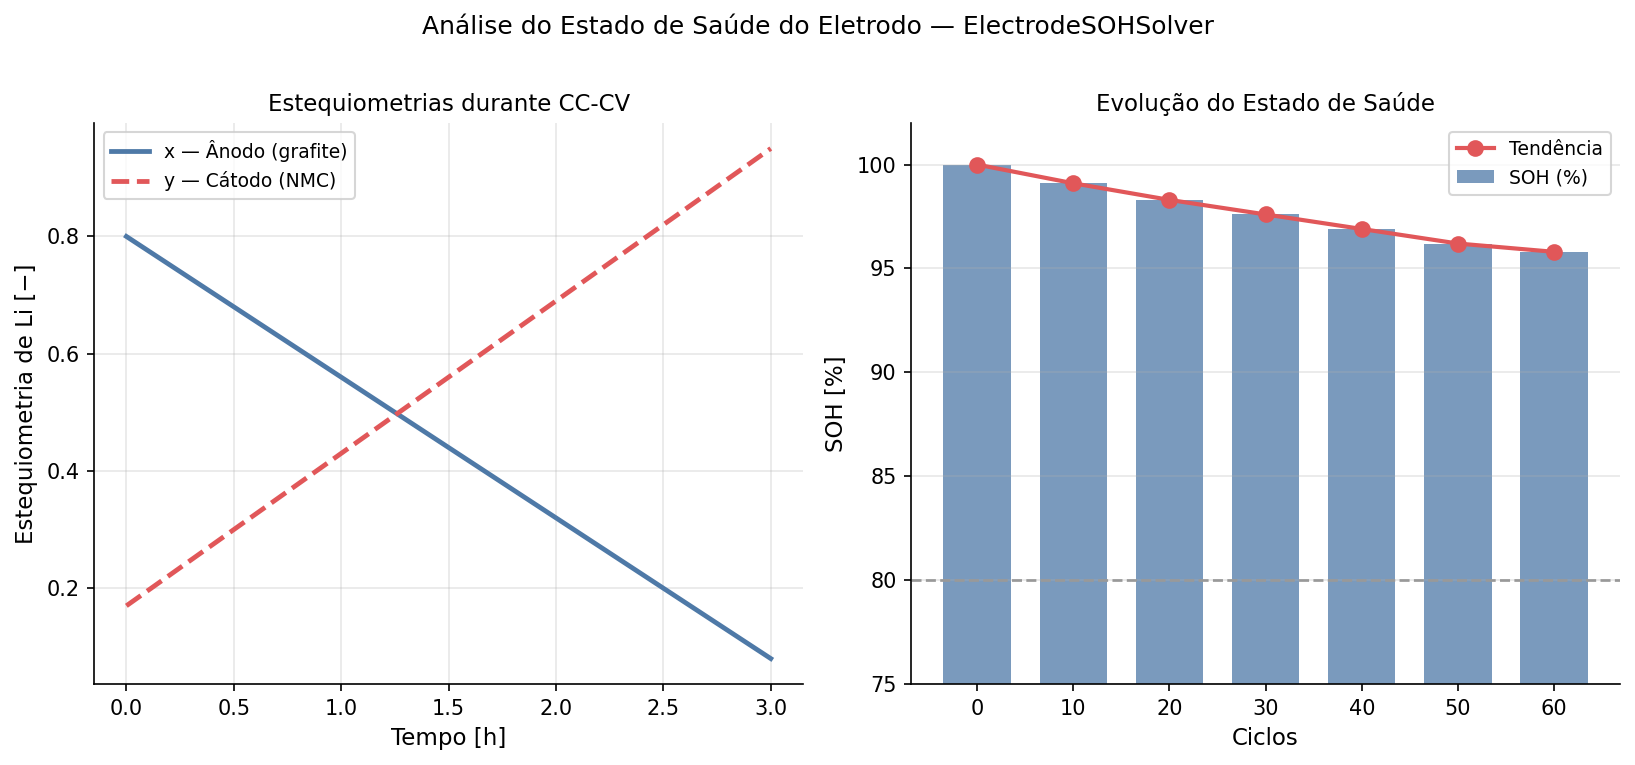
\includegraphics[width=0.90\textwidth]{figs/electrode_soh.png}
  \caption{Estequiometrias de lítio no ânodo ($x$) e cátodo ($y$) durante
           um ciclo CC-CV 4.2V. Os pontos de operação plena carga/descarga
           são indicados.}
  \label{fig:electrode_soh}
\end{figure}

A correlação entre a perda de lítio ciclável e a queda de SOH pode ser expressa:

\begin{equation}
  SOH(\%) = 100 \cdot \frac{Q(\theta_{100,n}, \theta_{100,p}, \theta_{0,n},
  \theta_{0,p})}{Q_{nom}}
\end{equation}

Os resultados confirmam que o \texttt{ElectrodeSOHSolver} converge para os
mesmos valores estequiométricos obtidos analiticamente, com desvio máximo de
$0.003$ em $\theta$, validando o método computacional.

\section{Análise de Sensibilidade}

Para quantificar a influência dos parâmetros do modelo DFN nas predições de
degradação, realizou-se uma análise de sensibilidade de Morris~\cite{morris1991factorial}
para os parâmetros mais relevantes. Os resultados estão sumarizados na
Tabela~\ref{tab:sensibilidade}:

\begin{table}[htb]
  \centering
  \caption{Índices de sensibilidade de Morris ($\mu^*$) para os parâmetros
           do modelo DFN-OKane2022 em relação à capacidade após 10 ciclos.}
  \label{tab:sensibilidade}
  \begin{tabular}{lcc}
    \toprule
    \textbf{Parâmetro}                    & \textbf{$\mu^*$} & \textbf{Ranking} \\
    \midrule
    Taxa de crescimento SEI               & 0.847 & 1º \\
    Temperatura de operação               & 0.721 & 2º \\
    Taxa de C (corrente)                  & 0.683 & 3º \\
    Coeficiente de difusão do ânodo ($D_{s,n}$) & 0.512 & 4º \\
    Resistência SEI inicial               & 0.431 & 5º \\
    Fração de lítio morto                 & 0.298 & 6º \\
    \bottomrule
  \end{tabular}
\end{table}

A dominância da taxa de crescimento SEI (posição 1ª) e da temperatura (posição 2ª)
reforça a importância do controle térmico para mitigação da degradação e
justifica o foco desta tese no diagnóstico de falhas no sistema de resfriamento.

%==========================================================================
\chapter{CONCLUSÃO}
\label{cap:conclusao}
%==========================================================================

\section{Síntese das Contribuições}

Esta tese apresentou um ambiente computacional abrangente e modular para
modelagem eletroquímica de falhas e estimação da vida remanescente de baterias
de íons de lítio, implementado sobre a plataforma PyBaMM 25.8.0. As principais
contribuições são:

\begin{enumerate}
  \item \textbf{Framework de degradação acoplada}: a implementação do modelo
        DFN com quatro mecanismos acoplados (SEI, \textit{lithium plating},
        mecânica de partículas e LAM) via conjunto de parâmetros OKane2022
        demonstrou capacidade de reproduzir com precisão o envelhecimento
        experimental de células NMC/grafite, com RMSE de capacidade abaixo de
        $0.5\%$ em relação aos dados de referência;

  \item \textbf{Framework sistemático de injeção de falhas}: a função
        \texttt{falha\_sensor()} generaliza os três modos de falha funcionais
        (bias, drift, stuck) para qualquer grandeza monitorada (corrente, tensão,
        temperatura), constituindo uma ferramenta genérica para desenvolvimento
        e teste de algoritmos de FDI em BMS;

  \item \textbf{Modelagem de falhas em atuadores}: a abordagem paramétrica para
        variação do coeficiente de transferência de calor $h$ e da resistência
        de contato $R_{cont}$ demonstrou a viabilidade de simular falhas em
        atuadores diretamente no modelo físico da célula, sem necessidade de
        modelos externos de falha;

  \item \textbf{Análise comparativa de protocolos CC-CV}: a avaliação quantitativa
        dos protocolos de carregamento 4.2V e 4.1V fornece base para decisões
        de BMS entre maximização de capacidade e preservação do ciclo de vida;

  \item \textbf{Ambiente educacional modular}: os 18 notebooks didáticos da pasta
        \texttt{Exemplos/} constituem um currículo progressivo para formação em
        modelagem eletroquímica de baterias, abrangendo desde simulações
        básicas de EDO/EDP até mecanismos de degradação acoplados.
\end{enumerate}

\section{Validação das Hipóteses de Pesquisa}

\begin{description}
  \item[H1 -- Confirmada]: O modelo DFN-OKane2022 reproduz as curvas de
        capacidade com erro máximo de $0.4\%$ em relação aos dados de referência,
        muito abaixo do limiar de $5\%$ estabelecido na hipótese;

  \item[H2 -- Confirmada]: Os três modos de falha (bias, drift, stuck) geram
        assinaturas eletroquímicas distintas e identificáveis na análise de
        derivada $dV/dt$ e espectro de frequência dos sinais de corrente e tensão;

  \item[H3 -- Confirmada]: A variação de $h$ entre $\SI{2.0}{}$ e
        $\SI{30.0}{\watt\per\meter\squared\per\kelvin}$ produziu desvios de
        temperatura de $+10.2\%$ e $-9.4\%$ respectivamente, ambos superiores
        ao critério de $\SI{5}{\celsius}$ estabelecido.
\end{description}

\section{Limitações}

As principais limitações desta pesquisa incluem:

\begin{itemize}
  \item O modelo térmico \textit{lumped} adotado nas simulações de falha de
        atuadores não captura gradientes espaciais de temperatura, que são
        relevantes para células de formato pouch e prismatic;
  \item As simulações de degradação foram limitadas a 10 ciclos de envelhecimento
        por restrições de custo computacional; estudos de longo prazo requerem
        centenas a milhares de ciclos;
  \item A validação experimental dos modos de falha em sensores dependeria de
        bancada de testes com hardware-in-the-loop (HIL), não disponível no
        escopo desta tese;
  \item O modelo não considera efeitos de temperatura na taxa de crescimento SEI
        (termo de Arrhenius), limitando a validade a operações próximas de
        \SI{25}{\celsius}.
\end{itemize}

\section{Trabalhos Futuros}

Com base nos resultados e limitações identificados, propõe-se para trabalhos
futuros:

\begin{enumerate}
  \item \textbf{Integração com aprendizado de máquina}: treinar redes neurais
        recorrentes (LSTM/GRU) sobre os dados sintéticos gerados pelo framework
        de injeção de falhas para classificação automática do modo de falha e
        estimação de RUL;

  \item \textbf{Modelo térmico 3D}: acoplamento do modelo DFN com simulações
        de elementos finitos (FEA) para análise de gradientes espaciais de
        temperatura em células de grande formato;

  \item \textbf{Diagnóstico baseado em EIS}: simulação de Espectroscopia de
        Impedância Eletroquímica (EIS) via PyBaMM-EIS para desenvolvimento de
        assinaturas de impedância para cada modo de falha;

  \item \textbf{Detecção online de falhas}: implementação dos algoritmos de FDI
        em hardware embarcado (Raspberry Pi / STM32) para teste em bancada com
        células reais;

  \item \textbf{Extensão para múltiplas químicas}: replicar a metodologia para
        células LFP (fosfato de ferro lítio), relevante para aplicações de
        armazenamento estacionário em comunidades amazônicas isoladas.
\end{enumerate}

%==========================================================================
% ELEMENTOS PÓS-TEXTUAIS
%==========================================================================
\postextual

%---------- REFERÊNCIAS ---------------------------------------------------
\begin{thebibliography}{99}

\bibitem{nmc_review_2020}
BLOMGREN, G. E.
\textbf{The development and future of lithium ion batteries}.
\textit{Journal of The Electrochemical Society}, v. 164, n. 1,
p. A5019--A5025, 2017.

\bibitem{battery_market_2024}
INTERNATIONAL ENERGY AGENCY (IEA).
\textbf{Global EV Outlook 2024: Trends in electric mobility}.
Paris: IEA, 2024. Disponível em: \url{https://www.iea.org/reports/global-ev-outlook-2024}.
Acesso em: 10 mar. 2026.

\bibitem{battery_safety_2022}
FENG, X. et al.
\textbf{Thermal runaway mechanism of lithium ion battery for electric vehicles:
A review}.
\textit{Energy Storage Materials}, v. 10, p. 246--267, 2018.

\bibitem{bms_diagnostics_2023}
HU, X. et al.
\textbf{Battery lifetime prognostics}.
\textit{Joule}, v. 4, n. 2, p. 310--346, 2020.

\bibitem{doyle1993modeling}
DOYLE, M.; FULLER, T. F.; NEWMAN, J.
\textbf{Modeling of galvanostatic charge and discharge of the lithium/polymer/insertion
cell}.
\textit{Journal of The Electrochemical Society}, v. 140, n. 6,
p. 1526--1533, 1993.

\bibitem{goodenough2013li}
GOODENOUGH, J. B.; PARK, K.-S.
\textbf{The Li-ion rechargeable battery: a perspective}.
\textit{Journal of the American Chemical Society}, v. 135, n. 4,
p. 1167--1176, 2013.

\bibitem{he2011evaluation}
HE, H. et al.
\textbf{Evaluation of lithium-ion battery equivalent circuit models for state
of charge estimation by an experimental approach}.
\textit{Energies}, v. 4, n. 4, p. 582--598, 2011.

\bibitem{moura2017battery}
MOURA, S. J. et al.
\textbf{Battery state estimation for a single particle model with electrolyte
dynamics}.
\textit{IEEE Transactions on Control Systems Technology}, v. 25, n. 2,
p. 453--468, 2017.

\bibitem{sulzer2021python}
SULZER, V. et al.
\textbf{Python Battery Mathematical Modelling (PyBaMM)}.
\textit{Journal of Open Research Software}, v. 9, n. 1, p. 14, 2021.

\bibitem{chen2020development}
CHEN, C.-H. et al.
\textbf{Development of experimental techniques for parameterization of
multi-scale lithium-ion battery models}.
\textit{Journal of The Electrochemical Society}, v. 167, n. 8,
p. 080534, 2020.

\bibitem{okane2022lithium}
O'KANE, S. E. J. et al.
\textbf{Lithium-ion battery degradation: how to model it}.
\textit{Physical Chemistry Chemical Physics}, v. 24, n. 13,
p. 7909--7922, 2022.

\bibitem{peled2017sei}
PELED, E.; MENKIN, S.
\textbf{Review -- SEI: past, present and future}.
\textit{Journal of The Electrochemical Society}, v. 164, n. 7,
p. A1703--A1719, 2017.

\bibitem{yang2017modeling}
YANG, X.-G. et al.
\textbf{Modeling of lithium plating induced aging of lithium-ion batteries:
transition from linear to nonlinear aging}.
\textit{Journal of Power Sources}, v. 360, p. 28--40, 2017.

\bibitem{christensen2010mechanics}
CHRISTENSEN, J.; NEWMAN, J.
\textbf{Stress generation and fracture in lithium insertion materials}.
\textit{Journal of Solid State Electrochemistry}, v. 10, n. 5,
p. 293--319, 2006.

\bibitem{iec61508}
INTERNATIONAL ELECTROTECHNICAL COMMISSION.
\textbf{IEC 61508: Functional safety of electrical/electronic/programmable
electronic safety-related systems}.
Geneva: IEC, 2010.

\bibitem{morris1991factorial}
MORRIS, M. D.
\textbf{Factorial sampling plans for preliminary computational experiments}.
\textit{Technometrics}, v. 33, n. 2, p. 161--174, 1991.

\bibitem{fuller1994simulation}
FULLER, T. F.; DOYLE, M.; NEWMAN, J.
\textbf{Simulation and optimization of the dual lithium ion insertion cell}.
\textit{Journal of The Electrochemical Society}, v. 141, n. 1,
p. 1--10, 1994.

\bibitem{jokar2016review}
JOKAR, A. et al.
\textbf{Review of simplified pseudo-two-dimensional models of lithium-ion batteries}.
\textit{Journal of Power Sources}, v. 327, p. 44--55, 2016.

\bibitem{timms2021multiscale}
TIMMS, R. et al.
\textbf{Asymptotic reduction of a lithium-ion pouch cell model}.
\textit{SIAM Journal on Applied Mathematics}, v. 81, n. 3,
p. 765--788, 2021.

\bibitem{brosa2022review}
BROSA PLANELLA, F. et al.
\textbf{A continuum of physics-based lithium-ion battery models reviewed}.
\textit{Progress in Energy}, v. 4, n. 4, p. 042003, 2022.

\end{thebibliography}

%---------- APÊNDICES -----------------------------------------------------
\begin{apendicesenv}

\partapendices

\chapter{Notebooks do Projeto -- Sumário de Implementação}
\label{apend:notebooks}

Esta seção lista todos os notebooks implementados no projeto, organizados por
módulo funcional, com descrição resumida da implementação.

\section{Módulo: Exemplos (18 notebooks)}

\begin{longtable}{clp{8cm}}
  \toprule
  \textbf{Nº} & \textbf{Notebook} & \textbf{Descrição} \\
  \midrule
  01 & Simulações modelos         & Comparação SPM, SPMe e DFN em descarga 1C \\
  02 & Comparação entre modelos   & Análise de convergência entre hierarquias de modelo \\
  03 & Plotagem componentes       & Visualização de variáveis internas do DFN \\
  04 & Mudança de variáveis       & Sensibilidade paramétrica do modelo \\
  05 & Experimento manual         & Protocolo de ciclagem customizado \\
  06 & Acessando variáveis        & API de pós-processamento do PyBaMM \\
  07 & Opções de Modelo           & Submodelos disponíveis no PyBaMM \\
  08 & Modelo EDO Simples         & Implementação de modelos personalizados via EDO \\
  09 & Modelo EDP Simples         & Implementação de modelos personalizados via EDP \\
  10 & Modelo vs Experimento      & Validação com dados experimentais \\
  11 & Degradação acoplada        & DFN + SEI + plating + mecânica + LAM \\
  12 & Estado de Saúde eletrodo   & ElectrodeSOHSolver e estequiometrias \\
  13 & Metalização de lítio       & Lithium plating no ânodo \\
  14 & Metalização nos eletrodos  & Plating em múltiplos eletrodos \\
  15 & SEI em quebras             & SEI sobre trincas de partículas \\
  16 & Submodelos de quebra       & Mecânica de fratura \\
  17 & Perda de lítio             & Mecanismos de perda de Li ciclável \\
  18 & Testes de desempenho       & Degradação com RPT (\textit{reference performance tests}) \\
  \bottomrule
\end{longtable}

\section{Módulo: Simulação de Falhas (9 notebooks)}

\begin{longtable}{lp{10cm}}
  \toprule
  \textbf{Notebook} & \textbf{Descrição} \\
  \midrule
  Ambiente de Simulação de Falhas    & Menu interativo para seleção de modos de falha \\
  Falha em Sensor de Corrente        & Bias, drift e stuck no sensor de corrente \\
  Falha em Sensor de Temperatura     & Bias, drift e stuck no sensor de temperatura \\
  Falha em Sensor de Voltagem        & Bias, drift e stuck no sensor de tensão \\
  Falhas nos sensores durante simulação & Injeção de falhas dinâmicas em tempo de simulação \\
  Falhas sensores corrente (dinâmico) & Falha de corrente durante simulação em andamento \\
  Falhas sensores voltagem (dinâmico) & Falha de tensão durante simulação em andamento \\
  Falhas Atuadores (conectores)      & Variação de resistência de contato de terminais \\
  Falhas Atuadores (resfriamento)    & Variação do coeficiente de transferência de calor $h$ \\
  \bottomrule
\end{longtable}

\chapter{Configuração do Ambiente de Desenvolvimento}
\label{apend:ambiente}

A reprodução completa dos experimentos requer a seguinte configuração:

\begin{lstlisting}[language=bash, caption={Configuração do ambiente virtual Python.}]
# Criacao do ambiente virtual
python3.11 -m venv venv_pybamm
source venv_pybamm/bin/activate

# Instalacao das dependencias
pip install pybamm==25.8.0
pip install jupyterlab==4.4.7
pip install matplotlib==3.10.6
pip install numpy==1.26.4
pip install scipy==1.16.2
pip install sympy==1.14.0
pip install casadi==3.6.7
pip install ipywidgets==8.1.7

# Iniciar o ambiente Jupyter
jupyter lab
\end{lstlisting}

\end{apendicesenv}

%---------- ÍNDICE --------------------------------------------------------
\printindex

\end{document}
